%%!TEX encoding = UTF-8 Unicode

\documentclass[oneside]{ntuthesis}

\usepackage[utf8]{inputenc}

% Use biblatex instead of bibtex
\usepackage[backend=bibtex, style=ieee]{biblatex}
%% Add all bib source files
\addbibresource{bib/articles.bib}
\addbibresource{bib/books.bib}
\addbibresource{bib/electronic.bib}
\addbibresource{bib/inproceedings.bib}
\addbibresource{bib/proceedings.bib}

\usepackage{mystyle}


%% Disable this package after finishing editing
\usepackage[disable]{todonotes}

% Type your personal information
%% Chinese
%\setUniversityZH  {國立臺灣大學} 
\setCollegeZH     {電機資訊學院}
\setInstituteZH   {電子工程學研究所}
\setThesisTypeZH  {碩士論文}
\setTitleZH		  {以PAC安全性保證實作程式測試}
\setAuthorZH      {李宗儒}
\setAdvisorNameZH {王~凡}
\setAdvisorTitleZH{博士}
%\setGradYearZH    {105} % The date is generated using \today
%\setGradMonthZH   {7}   % You can un-comment and specify the date

%% English
%\setUniversityEN  {National Taiwan University}
\setCollegeEN     {College of Electrical Engineering and Computer Science}
\setInstituteEN   {Graduate Institute of Electronics Engineering}
\setThesisTypeEN  {Master Thesis}
\setTitleEN		  {Program Testing with PAC Guarantees}
\setAuthorEN      {Lii, Tsung-Ju}
\setAdvisorNameEN {Farn Wang}
\setAdvisorTitleEN{Ph.D.}
%\setGradYearEN    {2015} % The date is generated using \today
%\setGradMonthEN   {June} % You can un-comment and specify the date


\begin{document}
\begin{CJK*}{UTF8}{bkai}

\frontmatter
\maketitle   % Generate title page

% Dummy chapter for generating ToC
%\addcontentsline{toc}{chapter}{口試委員會審定書}
%
\includepdf[pages={1},pagecommand={}]{official/approvalZH-with-sign}
%\addcontentsline{toc}{chapter}{Oral Examination Approval Form}
%
\includepdf[pages={1},pagecommand={}]{official/approvalEN-with-sign}

\begin{onehalfspace}

\chapter{Acknowledgements}
I should like to thank Prof. Yu-Fang Chen and Prof. Bow-Yaw Wang at Formal
Methods Laboratory in Academia Sinica.
Your guidance and instructions helped me gradually develop the whole framework
since I was a full-time research assistant in FM Lab.
Your solid training and teaching also forced me to establish my knowledge of
Software Verification and Formal Methods.
In particular, the opportunity and the experience you gave me to attend
international conferences surely is very enlightening though quite frightening.
In addition, I am specially grateful to and surprised by the assistance from
Dr. Ming-Hsien Tsai on the implementation.
Your efficiency and proficiency on software programming skills are simply
remarkable and incomparable.
Without your assistance, I am sure I cannot finish the implementation on my own,
let alone participating the competition.

I also learned a lot and pretty enjoyed my life in Software Testing Laboratory
in National Taiwan University.
Prof. Farn Wang is a great role model as a academic researcher.
His ambition on building an industrial strength software testing tool is
respectable.
The laboratory members and assistants are just adorable.
You guys inspired me in a unique way.
Even when we were both struggling for homeworks, reports, exams, and finally
the graduation, you guys still found many ways to relax and relief the tension
among the whole lab.
"Work Hard, Play Hard" is the spirit I learned from you.
You guys rock.

Finally, my appreciation to my parents and siblings is beyond words.
Thanks for your constant nagging on me about my physically and mentally
unhealthy lifestyle as well as trying to stop my 26-year-without-girlfriend
achievement.
Your concerns and considerations kept reminding me that,
even if I might fail so hard and be so frustrated, I still can go home,
where I can relax and recover until the next challenge comes.

\vspace{8mm}

\noindent
Thank you all.

\vspace{8mm}

\noindent
National Taiwan University, Taipei

\noindent
July, 2015 \hfill 謝橋 \ Hsieh, Chiao


\end{onehalfspace}

\begin{onehalfspace}
\newcommand{\eng}[1]{\ \raisebox{1pt}{#1}}

\chapter{摘要}
在程序分析 \eng{(Program Analysis)} 領域中,
分析遞迴程式 \eng{(Recursive Program)} 是一項難以處理的課題。
現有程式分析工具往往因為無法處理程式中的遞迴函式,
既而忽略部分程式碼不進行分析,或甚至拒絕檢驗遞迴程式。
本篇論文針對遞迴程式的分析提出新的觀點與分析方法;
作者認為與其重新設計演算法且實作新的分析器,
不如改進現有的程式分析工具。
但更改他人實作的軟體工具並非易事,
因此本文提出的方法將現有的工具視為黑箱不做任何更動,
反而是利用程式變換方法 \eng{(Program Transformation)} 將待分析的遞迴
程式轉換成無遞迴的程式,再交給黑箱分析工具進行檢驗;
並使用黑箱工具提供被分析程式中的不變量 \eng{(Invariants)},
進而證明原遞迴程式的正確性。

本篇作者與實驗室團隊受惠於程式分析工具 \eng{\textsc{CPAchecker}},
實作出此演算法的雛型 \eng{\textsc{CPArec}},
且參與 \eng{2015} 年度軟體驗證競賽 \eng{(Competition on Software Verification)};
和其它頂尖實驗室所開發工具相較,我們的工具針對遞迴程式進行分析時,
亦表現出相當的效率及效能,獲得第三名的佳績。

關鍵字:軟體驗證、程序分析、靜態分析、遞迴程式、程式變換方法

\end{onehalfspace}

\begin{doublespace}

\chapter{Abstract}

Recursion can complicate program analysis significantly.
Some program analyzers simply ignore recursion or even refuse to check recursive
programs.
In this paper, we propose an algorithm that uses a recursion-free program
analyzer as a black box to check recursive programs.
With extended program constructs for assumptions, assertions, and
non-deterministic values,
our algorithm computes function summaries from inductive invariants computed by
the underlying program analyzer.
Such function summaries enable our algorithm to check recursive programs.
We implement a prototype named \textsc{CPArec} using the recursion-free program
analyzer \textsc{CPAchecker}.
Under the comparison with other program analyzers on the benchmarks in the 2014
and 2015 Competitions on Software Verification,
our tool shows competitive efficiency and effectiveness on verifying programs
with recursion.

Key words: CPArec, Software Verification, Program Analysis, Static Analysis,
Recursion, Program Transformation

\end{doublespace}

\begin{doublespace}
\tableofcontents
\listoffigures
\listoftables
\todo[inline]{Add List of Symbols}
\end{doublespace}


\mainmatter
\begin{doublespace}

\chapter{Introduction}\label{ch:introduction}

Formal verification on software aims to prove program properties through rigorous mathematical reasoning. Consider, for example, the statement \texttt{assert(x > 0)} in C language. The statement explicitly asserts that the value of the variable \texttt{x} is positive. If the assertion is formally verified, it \emph{cannot} be violated in any possible execution during runtime. Formal verification techniques are, however, often computationally expensive. Although sophisticated heuristics have been developed in hopes of improving scalability of the techniques, formally verifying real-world software is still considered to be impractical. 

A common practice to ensure program quality in industry is software testing. Errors in software can be detected by exploring different software behaviors via injecting various testing vectors. On the other hand, software testing cannot guarantee a program to be free from errors. Consider again the assertion \texttt{assert(x > 0)}. Unless all system behaviors are explored by the testing vectors, it is unsound to conclude that the value of \texttt{x} is always positive. Various techniques have been proposed to improve its coverage, but it is an inherent feature of software testing that it cannot establish program properties conclusively. 

In this paper, we propose two approaches to repel the issues in the practices mentioned in the above paragraphs, namely the \emph{learning-based} procedure and the \emph{sampling-based} procedure. To be more specific, the approches we propose aim to balance the scalability and coverage of existing software engineering techniques. In order to be scalable, as for software testing, our technique only expores only a subset of all program behaviors. Moreover, in the learning-based procedure we apply machine learning to generalize observed program behavior for better sementic coverage. Our techniques allow software engineers to combine scalable testing with high-coverage formal analysis, while also improving the quality assuring process. In a nutshell, we hope our work can reduce the dichotomy between formal and practical software engineering techniques. 

In our techincal setting, we assume programs are annotated with program assertions. A program assertion is a Boolean expression intended to be true every time it is encountered during program execution. Given a program with assertions, our task is to check whether 
\emph{all} assertions evaluate to true on all a=possible executions. In principle, this problem can be solved by examining all program executions. However, it is clearly not possible to inspect every execution exhaustively, since there may be infinitely many of them. A method to simplify the analysis is to group the set of program executions to paths of a control flow graph. 

A \emph{control flow graph} (CFG) is derived from the syntactic structure of a program source code. Each execution of a program corresponds to a path in its control flow graph. Consequently, one can measure the completenes of software testing on CFGs. Line coverages, for instance, gives the ratio of explored edges in the CFG of the program-under-test, while branch coverage is the ratio of explored branches in the CFG. Note that such syntactic measures of code coverage approximate program executions only very roughly. Executions that differ in the number of iterations in a simple loop have the same line and branch coverages, although their computation may be drastically different. A full syntactic code coverage does not necessarily mean all execution paths have been explored by software testing.

Observe that program executions traversing the same path in a CFG performs the same sequence of operations (possibly with different values). Consider a path corresponding to a program execution in a CFG. Such a path can be characterized by the sequence of decisions taken by the execution while traversing the condition statements in the CFG. We call a sequence of such decisions a \emph{decision vector}. A decision vector is deemed feasible if it represents one or more, possibly infinitely many, program executions, and is infeasible if it represents a sequence of branching decisions that can never occur in the program executions. To check whether all assertions evaluate to true on all executions, if suffices to check only the set of all feasible decision vectors, and examine if any of them represents an assertion-violating program execution. Although feasibility of a decision vector can be determined by using a readily available Satisfiability Modulo Theories (SMT) solver, computing and generating the exact set of feasible decision vectors is difficult in general. In the learning-based procedure, we apply algorithmic learning, in particular the framework of \emph{probably approximately correct} (PAC) learning, to construct a regular approximation of this set. As for the sampling-based procedure, we utilize the correctness guarantee provided by the PAC learning framework, and use sampling to ensure program quality. 

\section{PAC Learning: An Introduction}\label{sec:intro_pac}

Within the framework of \emph{probably approximately correct} (PAC) learning with queries, learning algorithms query about target concepts to construct hypotheses. The constructed hypotheses are then validated by sampling. If a hypothesis is invalidated by a witness to a counterexample, learning algorithms refine the invalidated hypothesis by the witness and more queries. If, on the other hand, a hypothesis conoforms to all the samples, PAC learning algorithms return the inferred statistical guarantee with statistical guarantees. In this work, we adopt a PAC learning algorithm with queries to infer a regular language representive of the approximation to the set of feasible decision vectors of a program.

In the following paragraph, we will demonstrate an intuitive description of the statistical guarantee provided by PAC learning. Consider the task of checking defects in a large shipment. Moreover, the size of the shipment is so large such that it is impractical to check every item. We instead want to know if we can provide the guarantee, "the defect probability is at most $\epsilon$", with confidence of at least $\delta$, where $\epsilon$ and $\delta$ are given numbers and $\epsilon, \delta \in [0,1]$. This can be done by randomly selecting $r$ items, where $r$ is a number whose value is to be disclosed later. If all $r$ items are good, then our method reports that the defect probability is at most $\epsilon$. We argue the simple method can err with a probability of at most $1-\delta$. Suppose the $r$ randomly chosen items are tested without any defect, but the defect probability is, in fact, \emph{more than $\epsilon$}. Under the thesis, this would mean that when randomly picking items from the shipment, the probability of picking a good one is less than $1-\epsilon$. Consequently, the probability of picking $r$ items without encountering any defects is less than $(1-\epsilon)^r$. That is, the method is incorrect with probability less than $(1-\epsilon)^r$. Take $r$ such that $(1-\epsilon) < 1-\delta$. The simple method reports incorrect results with probability at most $1-\delta$; we equivalently say the result of the method is \emph{$\PAC$}.

Using a similar argument, it can be shown that our PAC learning algorithm returns a regular set approximating the set of feasible decision vectors of the program-under-test with error probability $\epsilon$ and confidence $\delta$, where $\epsilon$ and $\delta$ are chosen by the user. If the inferred set contains no decision vectors representing assertion violating program executions, our techniques concludes the verification with statistical guarantees about correctness. 

Our learning-based approach finds a balance between formal analysis and testing. Rather than exploring program behaviors exhaustively, our technique infers an approximation of the set of feasible decision vectors through queries and sampling. Although the set of feasible decision vectors is generally not computable, PAC learning with queries may still return a regular set of it along with a quantified guarantee. Such an approximate model with statistical guarantees can be useful for program verification. With the approximate model that is $\PAC$ and proved to be free from assertion violations, one can conclude that the program is also $\PAC$. On the other hand, the sampling-based procedure directly utilizes the statistical guarantees provided by PAC learning, and use sampling to ensure program correctness with respect to the sampling mechanism and distribution of the samples. The statistical guarantees are different from syntactic code coverages in software testing. Recall that our application of PAC learning works over decision vectors, which in turn represent program executions. If our procedures do not find any assertion violation, the statistical guarantees give software engineers a semantic coverage of the program executions. Along with conventional syntactic code coverages, such information may help software engineers evaluate the quality of software.

\section{Analysis and Diagnosis}\label{sec:analysis_diagnosis}

We constructed a prototype named \textsc{Pac-Man} (PAC learning-based Model synthesizer and ANalyzer) of our learning and sampling procedures based on program verifiers \textsc{CPAchecker, CBMC} and the concolic tester \textsc{Crest}. The prototype consists of two modes, the synthesize-and-verify mode and the direct mode, corresponding to the learning-based and the sampling-based procedure respectively. We evaluate our prototype on the benchmarks from the recursive and \todo{is using array-examples as benchmarks a good idea????} array-reach categories from SV-COMP 2015 \cite{svcomp15} and 2016 \cite{svcomp16}. The results are quite encouraging -- we can find all errors that can be found by \textsc{Crest}. As for the learning-based procedure, we also provide quantified guarantee accompanied by a faithful model for many examples that are challenging for program verifiers and concolic testers alike. This approximate model can be used for tasks such as verifying the same program with a different set of assertion failures, analyzing the behavior of the program, etc. We submitted a paper describing the learning-based approach \cite{ChenHLLTWW16} to the International Conference on Software Engineering (ICSE) 2016 \cite{icse2016}, and was successfully accepted. Additionally, we submitted the direct mode of \PACMAN to participate in SV-COMP 2016, and acquired promising results. 

Our contributions are summarized as follows:
\begin{itemize}
	\item We showed that PAC learning algorithm can be applied to synthesize an accurate model of the set of feasible decision vectors of a program. Such a model can be useful in many different aspects of program verification (cf. Chapter \ref{ch:discussion} for details). It is not hard to adopt our approach to handle different type of systems (e.g., black-box systems), and to obtain approximate models with a different level of abstraction (e.g., on a function call graph).
	\item We developed two procedures based on the PAC learning framework, both providing statistical guarantees while applying testing techniques. To be more specific, the procedures use testing to collect samples and to find bugs. The learning-based procedure then utilzie PAC learning algorithm to generalize the samples to obtain an accurate model of the program-under-test, which can be then analyzed by verification techniques for statistical guarantees, whereas the sampling-based procedure directly takes the guarantee provided by PAC learning, uses the concolic tester as a sampler to obtain the samples, and finally concludes on the program-under-test's correctness. 
\end{itemize}

\begin{comment}
Program verification is a grand challenge with significant impact in computer science.
Its main difficulty is in great part due to complicated program features such as concurrent execution, \hide{of threads,} pointers, \hide{with unbounded heap size,} recursive function calls, \hide{with recursions,} and unbounded basic data types~\cite{ClarkeJS05}. Subsequently,  is extremely tedious to develop a verification algorithm thitat handles all features. Researches on program verification typically address some of these features and simplify others. Verification tools however are required to support as many features as possible. Since implementation becomes increasingly unmanageable with additional features, incorporating algorithms for all features in verification tools can be a nightmare for developers.

One way to address the implementation problem is by reduction. If verifying a new feature can be transformed to existing features, development efforts can be significantly reduced.
In this paper, we propose an algorithm to extend intraprocedural (recursion-free) program analyzers to verify recursive programs. Such analyzers supply an \emph{inductive invariant} when a program is verified to be correct an/d support program constructs such as assumptions, assertions, and nondeterministic values. Our algorithm transforms any recursive program into recursion-free ones and invokes an intraprocedural program analyzer to verify properties about the generated recursion-free programs. The verification results allow us to infer properties on the given recursive program.

Our algorithm proceeds by iterations. In each iteration, it transforms the recursive program into a recursion-free program that \emph{under-approximates} the behaviors of the original and sends the under-approximation to an intraprocedural program analyzer. If the analyzer verifies the under-approximation, purported \emph{function summaries} for recursive functions are computed. Our algorithm then transforms the original recursive program into more recursion-free programs with purported function summaries. It finally checks if purported function summaries are correct by sending these recursion-free programs to the analyzer.

Compared with other analysis algorithms for recursive programs, our approach is very lightweight. It only performs syntactic transformation and requires standard functionalities from underlying intraprocedural program analyzers. Moreover, our technique is very modular. Any intraprocedural analyzer providing proofs of inductive invariants can be employed in our algorithm. With the interface between our algorithm and program analyzers described here, incorporating recursive analysis with existing program analyzers thus only requires minimal implementation efforts. Recursive analysis hence benefits from future advanced intraprocedural analysis with little cost through our~lightweight and~modular~technique.

We implement a prototype using \textsc{CPAchecker} (over 140 thousand lines of \textsc{Java} code) as the underlying program analyzer~\cite{BeyerK11}. In our prototype, 1256 lines of \textsc{OCaml} code are for syntactic transformation and 705 lines of \textsc{Python} code for the rest of the algorithm. 270 lines among them are for extracting function summaries. Since syntactic transformation is independent of underlying program analyzers, only about 14\% of code need to be rewritten should another analyzer be employed. We compare it with program analyzers specialized for recursion in experiments. Although \textsc{CPAchecker} does not support recursion, our prototype scores slightly better than the second-place tool \textsc{Ultimate Automizer} on the benchmarks in the 2014 Competition on Software Verification~\cite{svcomp14}.
Encouraged by the result, we submitted and successfully published our approach
on Static Analysis Symposium~\cite{ChenHTWW14}.
We further participated the 2015 Competition on Software
Verification~\cite{svcomp15} under the name \textsc{CPArec}~\cite{ChenHTWW15}.

\hide{
Notice that in order to simplify the implementation effort, we turned off important optimizations such as adjust block encoding provided in \textsc{CPAchecker}, the performance of the prototype can be even better with those optimizations turned on.
}

\noindent
\textbf{Organization:}
Chapter~\ref{ch:related} describes related works.
Preliminaries are given in Chapter~\ref{ch:preliminaries}.
We give an overview of our technique in Chapter~\ref{ch:overview}.
Technical contributions are presented in Chapter~\ref{ch:proving-via-transformation}.
Chapter~\ref{ch:experiments} reports experimental results.
Finally, some insights and improvements are discussed in Chapter~\ref{ch:conclusion}.

\hide{
Difference compared with Whale
In general, Whale tries to extend Lazy Abstraction to verify interprocedural program.
It mainly constructs an iARG with path conditions that can encode function calls and check for reachability of bug.
Also it introduces an extended covering relation over summaries of function calls to deal with recursion.
Our work, however, uses bounded times of unwinding to construct paths across functions,
and we find reasonable summaries for recursive functions when proving safety of program.

For guessing summaries, both Whale and our work use under-approximation of function calls.
In Whale, the under-approximation of a function call is constructed through exploring paths without function call in the called function.
In our work, the function call is unwound and transformed, and the exploration is achieved by the program analyzer we used.
With our method, we can create more precise under-approximation by unwinding more times before transforming.

For proving summaries, Whale and our work apply the Hoare rule of recursion. Whale defines the covering relation between summaries upon Hoare rule of consequence for proving. Our work, in other way, directly proves by the used program analyzer.
}

\end{comment}

\chapter{Related Works}\label{ch:related}

Exact automata learning algorithm was first proposed by Angluin \cite{Angluin87}, and later improved by \cite{Angluin87,RivestS93,KearnsV94,BolligHKL09}. The concept of probably approximately correct (PAC) learning was first proposed by Valiant in his seminal work \cite{Valiant84}. The idea of turning an exact learning algorithm to a PAC learning algorithm can be found in Section 1.2 of \cite{Angluin88}.

Applying PAC learning to testing has been considered before \cite{Walkinshaw11,GoldreichGR98}. The work in \cite{GoldreichGR98} considers a program that manipulates graphs and check if the output graph has certain properties such as bipartite, $k$-colorable, etc. Our work considers assertion checking, which is more general than the specialized properties. The work in \cite{Walkinshaw11} leans more towards the theoretical aspects of the problem. The author estimates the maximal number of queries required to infer a model of a black-box machine. The context is quite different, e.g., the work does not discuss how to sample according to some distribution efficiently to produce the desired guarantee (bounded path coverage) as we do in this paper. 

The $L^\ast$ algorithm has been used to infer the model of error traces of a program. In \cite{ChapmanCKKST15}, instead of decision vectors, the authors try to learn the sequences of function calls leading to an error. However, the teacher in this work is implemented using a bounded model checker, hence can only guarantee correctness up to a given bound. The author do not make use of the PAC learning mechanism as we did in this work. 

Both our approach and statistical model checking \cite{SenVA04,LegayDB10,ZulianiPC13} provide statistical guarantees. Statistical model checking assumes a given model, while our mechanism generates models of programs with statistical guarantee. Those models can be analyzed using various techniques and reused for verifying different properties.

We implemented a prototype tool called \textsc{Pac-Man} based on this work. In the implementation, we used several off-the-shelf software model checkers, \textsc{CPAchecker} \cite{BeyerK11}, \textsc{CBMC} \cite{ClarkeKL04}, \textsc{Predator} \cite{DudkaPV11}, and \textsc{SeaHorn} \cite{GurfinkelKKN15} to decide the feasibility of the program execution traces. Also, we have used two third-party libraries, namely \textsc{libALF} \cite{BolligKKLNP10} and \textsc{libAMoRE++} \cite{MatzMPTV95}, to perform the operations on automata. Moreover, we used C Intermediate Language (CIL) \cite{NeculaMRW02} \cite{cil} to perform program transformations. Last but not least, we used the concolic tester \textsc{Crest} \cite{BurnimS08} to sample from the targeet program. 

We submitted the prototype tool to participate in SV-COMP 2016 \cite{svcomp16}. In particular, our tool ranked \nth{5} in the recursive subcategory, and \nth{4} in the array-reach subcategory. 


\begin{comment}
Numerous intraprocedural analysis techniques have been developed over the years.
Many tools are in fact freely available (see, for instance,
\textsc{Blast}~\cite{BeyerHJM07}, \textsc{CPAchecker}~\cite{BeyerK11}, and
\textsc{UFO}~\cite{AlbarghouthiLGC12}).
Interprocedural analysis techniques are also available (see~\cite{RepsHS95,
BallR01,CousotCFMMMR05,CuoqKKPSY12,coverity,polyspace} for a partial list).
Recently, recursive analysis attracts new attention.
The Competition on Software Verification adds a new category for recursive
programs in 2014~\cite{svcomp14}.
Among the participants, \textsc{CBMC}~\cite{ClarkeKL04},
\textsc{Ultimate Automizer}~\cite{HeizmannCDEHLNSP13}, and
\textsc{Ultimiate Kojak}~\cite{ErmisNDHP14} are the top three tools for the
\textbf{recursive} category.

Inspired by \textsc{Whale}~\cite{AlbarghouthiGC12}, we use inductive invariants
obtained from verifying under-approximation as candidates of summaries.
Also, similar to \textsc{Whale}, we apply a Hoare logic proof rule for recursive
calls from~\cite{Oheimb99}.
However, our technique works on control flow graphs and builds on an
intraprocedural analysis tool.
It is hence very lightweight and modular.
Better intraprocedural analysis tools easily give better recursive analysis
through our technique.
\textsc{Whale}, on the other hand, analyzes by exploring abstract reachability
graphs.
Since \textsc{Whale} extends summary computation and covering relations for
recursion, its implementation is more involved.

Aside from recursion analysis, using program transformation to reduce program
features is not a new concept.
We learned this concept particularly from~\cite{LalR08,LalR09},
where a program transformation technique for checking context-bounded concurrent
programs to sequential analysis is developed.
\end{comment}



\chapter{Preliminaries}\label{ch:preliminaries}

\section{Program Model}\label{sec:model}

Let $\mathcal{X}$ be the set of program variables and $\mathcal{F}$ the set of function and predicate symbols. We use $\mathcal{X'}$ for the set $\{x'| x \in \mathcal{X}\}$. The set $\mathcal{T}[\mathcal{X}, \mathcal{F}]$ of \textit{transition formulae} consists of well-formed first-order logic formulae over $\mathcal{X}$, $\mathcal{X'}$, and $\mathcal{F}$. For a transition $f \in {T}[\mathcal{X}, \mathcal{F}]$ and $\mathit{n} \in \mathbb{N}$, we use $f^{\langle n \rangle}$ to denote the formula obtained from \textit{f} by replacing all its free variables, $x \in \mathcal{X}$ and $x' \in \mathcal{X'}$, with $x^{ \langle n \rangle }$ and $x^{\langle n+1 \rangle }$. 

\todo[inline]{Extend to program with multiple procedures and procedure calls}
We then consider a program that can be represented as a single procedure using a control flow graph. A \emph{control flow graph (CFG)} is a graph $G = (V, E, v_i, v_r, V_e, \mathcal{X}_{FP})$, where $V = V_b \cup V_s$ is a finite set of \emph{nodes} consisting of disjoint sets of \emph{branching} nodes $V_b$ and \emph{sequential} nodes $V_s$, $v_i \in V$, is the \emph{initial} node, $v_r$ is the \emph{return} node, $V_e \subseteq V$ is the \emph{error} nodes, $\mathcal{X}_{FP} \subseteq \mathcal{X}$ is the eset of formal parameters, and $E$ is a finite subset of \emph{edges} such that $E \subseteq V \times \mathcal{T[X,F]} \times V$. Also, the following conditions should hold in a CFG:
\begin{itemize}
	\item For any branching node $v_b \in V_b$, there are exactly two nodes $v_0' , v_1' \in V$ such that $(v_b, f_0, v_0'), (v_b, f_1, v_1') \in E$, where $f_0, f_1 \in \mathcal{T[X,F]}$ are transition formulae.
	
	\item For any non-returning sequential nodes $v_s \in V_s \setminus \{v_r\}$, there is exactly one node $v'$ with $(v, f, v') \in E$.
	
	\todo[inline]{Need to rephrase this one????}
	\item For the return node $v_r$, then for any $f \in \mathcal{T[X,F]}$, there is no $v' \in V$ such that $(v, f, v') \in E$ .
\end{itemize}
A node $v'$ is a \emph{successor} of $v$ if there is a transition $f \in \mathcal{T[X,F]}$ such that $(v, f, v') \in E$. Moreover, assume the two successors $v_0'$ and $v_1'$ of a branching node $v$ are ordered. Intuitively, the "1" is for the \emph{if} branch, while the "0" is for the \emph{else} branch. We then call $v_0'$ and $v_1'$ as the \emph{0-successor} and \emph{1-successor}. $f_0$ and $f_1$ are called \emph{0-transition} and \emph{1-transition} in the same manner. 

The definition of a CFG allows describing nondeterministic choices, which are used extensively to describe the environment. A nondeterministic choice from a branching node $v$ can be represented by defining both the 0-transition and the 1-transition formulae as $\bigwedge_{x \in \mathcal{X}} x = x'$.

A \emph{path} in a CFG $G$ is a sequence $\pi = \langle v_0, f_1, v_1, f_2, v_2, \dots , f_m, v_m \rangle$, such that $v_0 = v_i$ and $(v_j, f_{j+1}, v_{j+1}) \in E$ for every $j \in [0, m)$. The path $\pi$ is \emph{feasible} if the path formula $\bigwedge_{k=1}^m f_k^{\langle k \rangle}$ is satisfiable. It is an \emph{error} path if $v_j \in V_e$ for some $j \in [0,m)$. Our objective is to check if $G$ contains a \emph{feasible error path}.

A \emph{sequence} $w= a_1a_2a_3 \dots a_n$ with $a_j \in \{0,1\}$, where $j \in [0,m)$, is called a \emph{word} over \{0,1\}. The \emph{length} of $w$ is $|w|$, which is equivalent to $n$. The word with length 0 is an \emph{empty} word $\lambda$. We use $w[j]$ to denote the $j_th$ symbol $a_j$ in a word $w$. If $u, w$ are words over \{0,1\}, then we denote the \emph{concatenation} of $u$ and $w$ as $u \cdot w$. A \emph{language} $L$ over \{0,1\} is a set of words over \{0,1\}.

We now introduce the function \textsf{decision}, which maps a path $\pi$ of a CFG $G$ to a sequence of decisions made in the branching nodes traversed by $\pi$. Formally, \textsf{decision} is a function from paths to words over {0,1} defined recursively as follows:
\begin{multline*}
	\mathsf{decision}(\langle v_0, f_1, v_1, f_2, v_2, \dots, f_m, v_m \rangle) \\
	= \mathsf{decision}(\langle v_0, f_1 \rangle) \cdot \mathsf{decision}(\langle v_1, f_2, v_2, f_3, v_3, \dots, f_m, v_m \rangle)
\end{multline*}
where
\begin{equation*}
	\begin{array}{rcl}
		\mathsf{decision}(\langle v \rangle) & = & \lambda \\
		\mathsf{decision}(\langle v, f \rangle) & = & 
		\begin{cases}
			\lambda & \text{if } v \in V_s \\
			0 		& \text{if } v \in V_b \text{ and } \\
					& f \text{ is the 0-transition formula of }v \\
			1		& \text{if } v \in V_b \text{ and } \\
					& f \text{ is the 1-transition formula of }v 	 
		\end{cases}
	\end{array}
\end{equation*} 

For a path $\pi$, $\DEC(\pi)$ is the \emph{decision vector} of $\pi$. Consequently, we can define \emph{decision vectors} of a set of paths $\Pi$ as $\DEC(\Pi) = \{\DEC(\pi) | \pi \in \Pi\}$.

\section{Two Classes of Automata}\label{sec:automata}

A \emph{finite automaton} (with $\lambda$-moves) $A$ is a tuple $A = (\Sigma, Q, q_i, \Delta, F)$ consisting of a finite \emph{alphabet} $\Sigma$, a finite set of \emph{states}, an \emph{initial state} $q_i \in Q$, a \emph{transition relation} $\Delta \subseteq Q \times (\Sigma \cup \{\lambda\}) \times Q$, and a set of \emph{accepting states} $F \subseteq Q$. A transition $(q, \lambda, q') \in \Delta$ is a \emph{$\lambda$-transition}. A word $w$ over $\Delta$ is \emph{accepted} by $A$ if there are states $q_0, \dots, q_m \in Q$ and symbols $a_1, \dots, a_m \in (\Sigma \cup \{\lambda\})$, such that $w = a_1a_2 \dots a_m$, there is a transition $(q_j, a_{j+1}, q_{j+1}) \in \Delta$ for every $j \in [0,m)$, $q_0 = q_i$, and $q_m \in F$. The \emph{language} of $A$ is defined as $L(A) = \{w|w \text{ is accepted by } A\} $. A language $R$ is regular if $R = L(A)$ for some finite automaton $A$. The finite automaton $A$ is \emph{detereministic} if its transition relation is a function from $Q \times \Sigma$ to $Q$. For any finite automaton A, there exists a deterministic finite automaton (DFA) $B$ such that $L(A) = L(B)$. 

A \emph{pushdown automaton} (PDA) is a tuple $P = (\Sigma, Q, \Gamma, q_i, \Delta, F)$ consisting of a finite \emph{input alphabet} $\Sigma$, a finite set of \emph{states} $Q$, a finite \emph{stack alphabet} $\Gamma$, an \emph{initial state} $q_i \in Q$, a set of \emph{finite states} $F \subseteq Q$, and \emph{transition relation} $\Delta \subseteq Q \times (\Sigma \cup \{\lambda\}) \times (\Gamma \cup \{\lambda\}) \times (\Gamma \cup \{\lambda\}) \times Q$. We use $(q, [a;b/c], q')$ to denote the transition $(q, a, b, c, q')$, and we simplify $(q, [a;\lambda/\lambda], q')$ to $(q, a, q')$. A \emph{configuration} of $P$ is a tuple $(q,\gamma) \in Q \times \Gamma^*$. A word $w$ over $\Sigma$ is \emph{accepted} by $P$ if there is a sequence of configurations $(q_0, \gamma_0), \dots, (q_m, \gamma_m) \in Q \times \Sigma^*$ and a sequence of symbols $a_1, \dots, a_m \in (\Sigma \cup \{\lambda\})$, such that $w=a_1a_2\dots a_m, q_0 = q_i, \gamma_0 = \epsilon, q_m \in F$, and for every $j \in [0,m)$ there are some $b_j, b_{j+1} \in (\Gamma \cup \{\lambda\})$ and $\gamma'_j, \gamma'_{j+1} \in \Gamma^*$ such that $\gamma_j = b_j\gamma'_j, \gamma_{j+1} = b_{j+1}\gamma'_{j+1}$, and there is $(q_j, [a_{j+1};b_j/b_{j+1}], q_{j+1}) \in \Delta$. The language of $P$ is defined as $L(P) = \{w | w \text{ is accepted by } P\}$.

\section{Concolic Testing}\label{sec:concolic_testing}

\emph{Concolic testing} \cite{GodefroidKS05,SenMA05} is a testing approach that explores paths in the CFG of a program while searching for bugs. The concolic tester begins its task by generating a decision vector by randomly picking the program's input values. Then, the tester finds the next decision vector by negating some decision made in the chosen decision vector, thus obtaining a new decision vector. The selection of which decision should be negated depends on the used \emph{search strategy} of the tester. The program then executes along the corresponding new path. This testing approach gives paths with rare paths a much greater chance to be explored. 

Below is an example to show the main distinction between classical random testing techniques and concolic testing. Consider the following program and its corresponding CFG (figure \ref{figure:concolic_testing}): 
\begin{lstlisting}[language=C]
void func(int x, int y){
   if (x == 2147483647) { 
      if (y >= x) { assert(0); /* error */ }
   }
}
\end{lstlisting}

\begin{figure}[h]
	\centering
	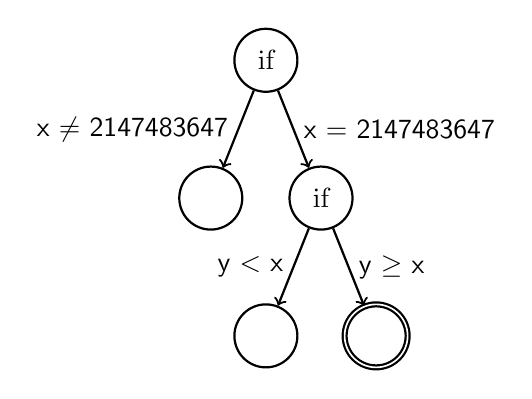
\begin{tikzpicture}[scale=0.7,->, auto, node distance=2cm, thick, node/.style={circle, draw, minimum width=0.8cm, inner sep=0pt},  accepting/.style={double, circle, draw, minimum width=0.8cm, inner sep=0pt}]
		\node[node] (0) at (0,0) {if};
		\node[node] (1) at (1,-2.5) {if};
		\node[node] (2) at (-1,-2.5) {};
		\node[node] (3) at (0,-5) {};
		\node[accepting] (4) at (2,-5) {};
		\path
		(0) edge node [right] {\textsf{x = 2147483647}} (1)
		edge node [left] {\textsf{x $\neq$ 2147483647}} (2)
		(1) edge node [left] {\textsf{y $<$ x}} (3)
		edge node [right] {\textsf{y $\geq$ x}} (4);	
	\end{tikzpicture}
	\caption{CFG of $\fun{func}$}
	\label{figure:concolic_testing}
\end{figure}
Random testing techniques would inject random values into $x$ and $y$. Since $x$ and $y$ are 32-bit integers, they can both take value in the range $[-(2^{31}), 2^{31}-1]$. However, only one combination in the $2^{128}$ possible ones, $x = 2147483647 \text{ and } y = 2147483647$, can reach the \texttt{assert(0);} in the function \texttt{func}. Concolic testing, on the contrary, only needs three tests to reach the error: since the concolic tester traverses the paths in the CFG, which in our case has three paths, it's clear that the concolic tester can reproduce the error within three tests. 

\begin{comment}

We consider a variant of the WHILE language from~\cite[Sec. 1.2]{NielsonHC99}:
\begin{equation*}
  \begin{array}{rccll}
    \mathtt{Expression} & \ni p & ::= &
    \mathtt{x} & \mathtt{x} \in \mathtt{Vars}\\
    & & \mid &
    \FF\ \mid\ \TT\ \mid\
    \mathtt{0}\ \mid\ \mathtt{1}\ \mid\ \ldots\hspace{5mm} &
    \textmd{constant}\\
    & & \mid &
    \mathtt{nondet} & \textmd{nondeterministic value}\\
    & & \mid &
    \fun{f}(\overline{p}) &
    \textmd{function invocation}\\
    & & \mid &
    p \odot p  & \odot \in \{ +, -, =, >, \mathtt{and}, \mathtt{or} \}\\
    & & \mid & \mathtt{not}\ p\\
    \mathtt{Command} & \ni c & ::= &
    \overline{\mathtt{x}} := \overline{p}
    & \textmd{assignment}\\
    & & \mid &
    c\mathtt{;}\ c &
    \textmd{sequential composition}\\
    & & \mid &
    \mathtt{return}\ \overline{p} & \textmd{function return}\\
    & & \mid &
    \mathtt{assume}\ p & \textmd{assumption}\\
    & & \mid &
    \mathtt{assert}\ p & \textmd{assertion}
  \end{array}
\end{equation*}
$\mathtt{Vars}$ denotes the set of \emph{program variables}, and
$\mathtt{Vars}' = \{ \mathtt{x}' : \mathtt{x} \in \mathtt{Vars} \}$
where $\mathtt{x}'$ represents the new value of $\mathtt{x}$ after
execution of a command.
%Let $t_i$ denote the $i$-th element in the sequence $\overline{t}$.
The $\mathtt{nondet}$ expression evaluates to a type-safe
nondeterministic value.
Simultaneous assignments are allowed in our language. To
execute a simultaneous assignment, all expressions on the right hand
side are first evaluated and then assigned to respective variables.
We assume that simultaneous assignments are type-safe in the sense that the
number of variables on the left-hand-side always matches that of the
right-hand-side.
The $\mathtt{return}$ command accepts several expressions as arguments.
Together with simultaneous assignments, functions can have several
return values.

\todo[inline]{Set restrictions on CFG to prevent arbitrary edges on graph
since the behavior may be undefined.}

A program \prog{P} is simply a set of functions.
Each function $\fun{f}$ in the program \prog{P} is represented as a
\emph{control flow graph (CFG)} $G^{\fun{f}} = \langle V, E, \cmd{cmd}^{\fun{f}},
\overline{\mathtt{u}}^{\fun{f}}, \overline{\mathtt{r}}^{\fun{f}}, s, e \rangle$
where the nodes in $V$ are \emph{program locations}, $E \subseteq V \times V$
are \emph{edges},
each edge $(\ell, \ell') \in E$ is labeled by the command $\cmd{cmd}^{\fun{f}}
(\ell, \ell')$,
$\overline{\mathtt{u}}^{\fun{f}}$ and $\overline{\mathtt{r}}^{\fun{f}}$ are
\emph{formal parameters} and \emph{return variables} of $\fun{f}$,
and $s,  e \in V$ are the \emph{entry} and \emph{exit} locations of $\fun{f}$.
The superscript in $G^{\fun{f}}$ denotes the CFG corresponds to the function
$\fun{f}$.
The special $\fun{main}$ function specifies where a program starts.
To simplify presentation, we assume the functions in a program use disjoint sets
of variables and the values of formal parameters never change in a function.
Notice that this will not affect the expressiveness of a CFG because one can
still make copies of formal parameters by assignments and change the values of
the copied versions.
Also we assume that there are no global variables because they can be simulated
by allowing simultaneous assignment to return variables~\cite{BallR00}.

Figure~\ref{figure:mccarthy91} shows control flow graphs for the
McCarthy 91 program from~\cite{MannaP70}. The $\fun{main}$ function assumes the
variable $\mathtt{n}$ is non-negative.
It then checks if the result of $\mathtt{mc91(n)}$ is no less than 90
(Figure~\ref{figure:mccarthy91:main}).
The $\fun{mc91}$ function branches on whether the variable $\mathtt{m}$ is
greater than 100.
If so, it returns $\mathtt{m} - 10$.
Otherwise, $\mathtt{mc91(m)}$ stores the result of $\mathtt{mc91(m + 11)}$
in $\mathtt{s}$,
and returns the result of $\mathtt{mc91(s)}$
(Figure~\ref{figure:mccarthy91:mc91}).
Observe that a conditional branch is modeled with the $\mathtt{assume}$ command
in the figure. Loops can be modeled similarly.

\begin{figure}
  \centering
  \begin{subfigure}[b]{.35\textwidth}
    \begin{tikzpicture}[scale=1.2,->,>=stealth',shorten >=1pt,auto,node
      distance=2cm,thick,node/.style={circle,draw,minimum width=0.8cm,inner sep=0}]
      \node[node,label=above:$\fun{main()}$] (0) at (0, 0) {$s$};
      \node[node] (1) at (0, -1) {$1$};
      \node[node] (2) at (0, -2) {$2$};
      \node[node] (3) at (0, -3) {$3$};
      \node[node] (4) at (0, -4) {$e$};

      \path
        (0) edge
            node [left] {$\mathtt{assume\ n >= 0}$} (1)
        (1) edge
            node [left] {$\mathtt{r := mc91(n)}$} (2)
        (2) edge
            node [left] {$
              \begin{array}{l}
                \mathtt{assert\ {[}r = 91\ or}\\
                \mathtt{\ \ \ \ \ \ \ \ \ \ \ (n > 101\ and\ \ }\\
                \mathtt{\ \ \ \ \ \ \ \ \ \ \ \ r = n - 10){]}}
              \end{array}$} (3)
        (3) edge
            node [left] {$\mathtt{return\ 0}$} (4);
    \end{tikzpicture}
    \caption{$\fun{main}$}
    \label{figure:mccarthy91:main}
  \end{subfigure}
  ~
  \begin{subfigure}[b]{.62\textwidth}
    \begin{tikzpicture}[scale=1.2,->,>=stealth',shorten >=1pt,auto,node
      distance=2cm,thick,node/.style={circle,draw,minimum width=0.8cm,inner sep=0}]
      \node[node,label=above:$\fun{mc91(n)}$] (0) at ( 0,  0) {$s$};
      \node[node] (1) at (-1, -2) {$1$};
      \node[node] (2) at ( 1, -0.8) {$2$};
      \node[node] (3) at ( 1, -2) {$3$};
      \node[node] (4) at ( 1, -3.2) {$4$};
      \node[node] (5) at ( 0, -4) {$e$};

      \path
        (0) edge [bend right=30]
            node [left] {$\mathtt{assume\ m > 100}$} (1)
            edge [bend left=30]
            node [right] {$\mathtt{assume\ not(m > 100)}$} (2)
        (1) edge [bend right=30]
            node [left] {$\mathtt{return\ m - 10}$} (5)
        (2) edge
            node [right] {$\mathtt{s := mc91(m + 11)}$} (3)
        (3) edge
            node [right] {$\mathtt{t := mc91(s)}$} (4)
        (4) edge [bend left=30]
            node [right] {$\mathtt{return\ t}$} (5);
    \end{tikzpicture}
    \caption{$\fun{mc91}$}
    \label{figure:mccarthy91:mc91}
  \end{subfigure}
  \caption{McCarthy 91}
  \label{figure:mccarthy91}
\end{figure}

\todo[inline]{Extend the definition of inductive invariants to support
interprocedural analysis}
% \section{Inductive Invariants}\label{sec:semantics}

Let $G^{\fun{f}} = \langle V, E ,\cmd{cmd}^{\fun{f}},
\overline{\mathtt{u}}^{\fun{f}}, \overline{\mathtt{r}}^{\fun{f}},  s,
e \rangle$ be a CFG.
An \emph{inductive invariant} $\Pi (G^{\fun{f}},I_0) = \{ I_\ell : \ell \in V \}$
for $G^{\fun{f}}$ from $I_0$ is a set of first-order logic formulae such that
$I_s = I_0$, and for every $(\ell, \ell') \in E$
\begin{equation*}
I_{\ell} \wedge \tau_{\cmd{cmd}^\fun{f}(\ell, \ell')} \implies I'_{\ell'}
\end{equation*}
where $I'$ is obtained by replacing every $\mathtt{x} \in \mathtt{Vars}$ in $I$
with $\mathtt{x}' \in \mathtt{Vars}'$,
and $\tau_{\cmd{cmd}^\fun{f} (\ell, \ell')}$ specifies the semantics of the
command $\cmd{cmd}^\fun{f} (\ell, \ell')$.
An inductive invariant $\Pi (G^{\fun{f}}, I_0)$ is an over-approximation to the
computation of $G^{\fun{f}}$ from $I_0$.
More precisely, assume that the function ${\fun{f}}$ starts from a state
satisfying $I_0$.
For every $\ell\in V$, $G^{\fun{f}}$ must arrive in a state satisfying
$I_{\ell}$ when the computation reaches $\ell$.

\todo[inline]{More about operational semantics?}

% \section{Hoare Logic and Program Analysis}\label{sec:analysis}

Let $T$ be a program fragment (it can be either a function represented as a CFG
or a sequence of program commands).
$P$ and $Q$ are logic formulae.
A \emph{Hoare triple} $\assert{P} T \assert{Q}$ specifies that the program
fragment $T$ will reach a program state satisfying $Q$ provided that $T$ starts
with a program state satisfying $P$ and terminates.
The formula $P$ is called the \emph{precondition} and $Q$ is the
\emph{postcondition} of the Hoare triple.
For intraprocedural commands, we extend the standard proof rules for partial
correctness in~\cite[Sec. 9.2]{NielsonN07} with two additional rules for the
assumption and assertion commands:
\begin{center}
  \AxiomC{}
  \LeftLabel{Assume}
  \UnaryInfC{$\assert{P}\ \mathtt{assume\ } q\
    \assert{P \wedge q}$}
  \DisplayProof
  ~
  \AxiomC{$P \implies q$}
  \LeftLabel{Assert}
  \UnaryInfC{$\assert{P}\ \mathtt{assert\ } q\  \assert{P}$}
  \DisplayProof
\end{center}
The $\mathtt{assume}$ command excludes all computation not satisfying the given
expression.
The $\mathtt{assert}$ command aborts the computation if the given expression is
not implied by the precondition.
No postcondition can be guaranteed in such a case.
For interprocedural analysis, we adopt the proof rules from~\cite{Oheimb99} for
(recursive) function calls.
In addition, there are other rules, e.g., the rules for unconditional
jumps~\cite{TanA06}.
However, those proof rules are not involved in our proof for correctness,
we consider them to be out of scope.

%For instance, the following command always terminates normally:
%\begin{equation*}
% \mathtt{assume\ false};\ \ \mathtt{assert\ false}
%\end{equation*}
Observe that an inductive invariant $\Pi (G^{\fun{f}}, I_0)$ establishes
$\assert{I_0} G^{\fun{f}} \assert{I_{e}}$.
A \emph{program analyzer} accepts programs as inputs and checks if all
assertions (specified by the $\mathtt{assert}$ command) are satisfied.
One way to implement program analyzers is to compute inductive invariants.
\begin{proposition}
Let $G^{\fun{f}} = \langle V, E,\cmd{cmd}^{\fun{f}},
\overline{\mathtt{u}}^{\fun{f}}, \overline{\mathtt{r}}^{\fun{f}}, s, e \rangle$
be a CFG and $\Pi (G^{\fun{f}}, \TT)$ be an inductive invariant for
$G^{\fun{f}}$ from $\TT$.
If $\models I_{\ell} \implies B_{\ell}$ for every edge $(\ell, \ell') \in E$
with $\cmd{cmd} (\ell, \ell') = \mathtt{assert} (B_{\ell})$,
then all assertions in $G^{\fun{f}}$ are satisfied.
\label{proposition:inductive-invariant}
\end{proposition}
A program analyzer which checks assertions by computing inductive invariants is
called an \emph{inductive} program analyzer.
Note that an inductive program analyzer need not give any information when an
assertion fails.
Indeed, most inductive program analyzers simply report false positives when
inductive invariants are too coarse.
%A \emph{program checker} is
%a program analyzer that returns an error trace when an assertion
%fails; an \emph{error trace} is a sequence of variable valuations from
%the program entry to the failed assertion. Rather than reporting false
%positives, program checkers have to return error traces to witness
%failed assertions. %Producing error traces (especially for recursive
%programs) complicates analysis algorithms. We hence consider a
%subclass of program checker.
A \emph{recursion-free inductive program analyzer} is a program analyzer that
checks recursion-free programs by computing inductive invariants.
Several recursion-free inductive program analyzers are available, such as
\textsc{CPAchecker}~\cite{BeyerK11}, \textsc{Blast}~\cite{BeyerHJM07},
\textsc{UFO}~\cite{AlbarghouthiLGC12}, \textsc{Astr\'ee}~\cite{CousotCFMMMR05},
etc.
Our goal is to check recursive programs by using a recursion-free inductive
program analyzer as a black box.
\end{comment}

\chapter{Overview}\label{ch:overview}

Let $G$ be a CFG of a program. Our objective is to determine whether a feasible error path exists in $G$. In a more formal convention, consider the set of feasible paths $\Pi \subseteq G$ and the set of error paths $\mathcal{B} \subseteq G$. We call the languages $\DEC	(\Pi)$ and $\DEC(\mathcal{B})$ over the alphabet $\{0,1\}$ as \emph{feasible decision vectors} and \emph{error decision vectors} respectively. If there are no feasible paths that are also error paths, then we can deduce the program is correct, since no feasible path in $G$ can reach any error node $v \in V_e$. In other words, the program is correct if $\DEC(\Pi) \cap \DEC(\mathcal{B}) = \emptyset$. 

Representing $\DEC(\Pi)$, the language of all feasible decision vectors in $G$, is actually quite challenging. In general, this language might not be regular or even computable. In our procedure, we construct a candidate finite automaton $C$ that approximates $\DEC(\Pi)$. Such a candidate automaton is constructed using a \emph{probably approximately correct} (PAC) online automata learning algorithm. PAC learning provides statistical guarantees about the correctness of $C$: $C$ is \emph{$\PAC$}, i.e., with \emph{confidence} $\delta$, the deviation of $L(C)$ from $\DEC(\Pi)$ is less than \emph{error rate} $\epsilon$. A more formal explanation of the terms and reasonings within the PAC learning framework is given in Chapter \ref{ch:PAC}.

Constructing a finite automaton $B$ that accepts the set of all error decision vectors $\DEC(\mathcal{B})$ is much more straightforward in comparison. Intuitively, states of $B$ corresponds to nodes in $G$, the initial state of $B$ corresponds to the initial node of $G$, and the final states of $B$ corresponds to $G$'s error nodes. An edge from a sequential node is mapped to a $\lambda$-transition, and the edges from a branching node to its 0- and 1-successors are mapped over symbols 0 and 1 respectively. We will go into the details of this construction in Chapter \ref{ch:error}.

\begin{figure}
	\centering
	\begin{tikzpicture}[node distance = 2cm, auto]
	\newcommand{\MEM}[0]{\mathit{Mem.}}
	\newcommand{\EQ}[0]{\mathit{Eq.}}
	\tikzstyle{decision} = [diamond, draw, fill=blue!20,
	text width=2.5cm, text centered, inner sep=0pt]
	\tikzstyle{block} = [rectangle, draw, fill=blue!20, 
	text centered, rounded corners, minimum height=0.8cm]
	\tikzstyle{line} = [draw, -latex'];
	
	% Draw Boxes
	
	\draw[rounded corners, fill=green!20]
	(0cm,1cm) rectangle +(6cm,-2cm);
	\node[text centered, text width=6cm] 
	at (3cm,0cm) {\textbf{PAC Automata Learning Algorithm}\\(Chapter \ref{ch:PAC})};
	\draw[rounded corners, fill=yellow!20]
	(0cm,6cm) rectangle +(6cm,-4cm);    
	\node[text badly centered, text width=6cm] at (3cm,5.4cm)
	{\textbf{Mechanical Teacher}};
	\draw[rounded corners, fill=blue!20]
	(0.3cm,5cm) rectangle +(2.5cm,-2.6cm);
	\node[text badly centered, text width=6cm] at (1.55cm,3.7cm) 
	{\text{Resolving}\\
		\text{Membership} \\
		\text{Queries} \\
		\text{(Chapter \ref{ch:mem})}};
	\draw[rounded corners, fill=blue!20]
	(3.2cm,5cm) rectangle +(2.5cm,-2.6cm);
	\node[text badly centered, text width=6cm] at (4.45cm,3.7cm) 
	{\text{Resolving}\\
		\text{Equivalence} \\
		\text{Queries} \\
		\text{by Sampling} \\
		\text{(Chapter \ref{ch:eq})}};
	\draw[rounded corners, fill=red!20]
	(-0.3cm,9.2cm) rectangle +(3cm,-2.9cm);
	\node[text badly centered, text width=6cm] at (1.2cm,7.75cm)
	{\text{Feasible} \\
		\text{Error} \\
		\text{Decision} \\
		\text{Vector} \\
		\text{Found}};
	\draw[rounded corners, fill=cyan!20]
	(3.1cm,9.2cm) rectangle +(3.6cm,-2.9cm);
	\node[text badly centered, text width=6cm] at (4.9cm,7.75cm)
	{\text{System is}\\
		$\PAC$};
	
	% Draw Arrows
	
	\path [line] (1,1) -- node {$\MEM(w)$} (1,2.4);
	\path [line] (1.5,2.4) -- node {yes/no} (1.5,1);
	\path [line] (4.5,1) -- node {$\EQ(C)$} (4.5,2.4);
	\path [line] (5,2.4) -- node {yes/counterexample} (5,1);
	\path [line](0,0) -- (-1,0) -- (-1, 7.25) -- (-0.3, 7.25);
	\path [line](5.7,4.2) -- (7.2,4.2) -- (7.2, 7.25) -- (6.7, 7.25);
	\path [line](5.7,3.2) -- (7.7,3.2) -- (7.7, 9.7) -- (1.2, 9.7) -- (1.2, 9.2);
	\end{tikzpicture}
	\caption{Components of our learning procedure}
	\label{figure:overview}
\end{figure}

An overview of our learning procedure is given in Figure \ref{figure:overview}. This procedure is actually similar in structure to the one of \cite{Angluin87}. There are two main components in the procedure: the \emph{teacher} and the \emph{learning algorithm}. The learning algorithm presents two queries to the teacher: \emph{membership query} ("Is a given decision vector feasible in the program?") and \emph{equivalence query} ("Is a given candidate finite automaton $\PAC$?"). The teacher is omniscient on the program behaviors, thus is able to resolve the queries correctly. Also, the teacher is able to test whether a decision vector is actually an error decision vector. By posing these queries, either the learning algorithm iteratively constructs a $\PAC$ approximation of the program, or our procedure finds a feasible error decision vector.

As with other online learning-based techniques, we need to devise a mechanical teacher that resolves queries presented by the learning algorithm. Resolving membership queries (i.e., membership in the set of feasible decision vectors $\DEC(\Pi)$) is relatively simple. For example, when given a decision vector $d$, we can obtain its corresponding path $\pi$ by unfolding the CFG $G$ according to $d$, and use an off-the-shelf solver to decide whether $\pi$ is feasible or not. (See Chapter \ref{ch:mem})

When the automata learning algorithm infer a candidate finite automaton $C$, we need to check whether $L(C)$ approximates $\DEC(\Pi)$, i.e., whether $C$ is $\PAC$. Since comparing $L(C)$ directly with $\DEC(\Pi)$ is not practical, we employ the sampling-based approximate equivalence technique of PAC learning. While being generally unsound, this technique still provides statistical guarantee about the correctness of the inferred candidate automaton. More details on how equivalence queries are made can be found in \ref{ch:eq}. The details of our learning-based procedure is in Chapter \ref{ch:learning_proc}. 

\todo[inline]{Sampling-based procedure... done by me... probably not very well written?}
In addition to the learning-based procedure, we propose a sampling-based procedure that provides the same statistical guarantees to a program, while excluding the overhead from constructing a candidate automaton in the learning-based procedure. Although the learning-based procedure can synthesize a program model that can be reused for different analyses, it comes with additional cost for model synthesis. The idea behind the sampling-based procedure is also based on PAC learning, but since no effort is spent on constructing a candidate automaton, the statistical guarantees provided by the sampling-based procedure can be much tighter than the learning-based procedure when given the same amount of computational resources. More descriptions on the sampling-based procedure is in \ref{ch:sampling_proc}.

Let \method{BasicAnalyzer} denote a recursion-free inductive program analyzer,
and let a program $\prog{P}=\{G^{\fun{main}}\}\cup\{G^{\fun{f}} : \fun{f}\mbox{ is a function}\}$
consist of the CFGs of the $\fun{main}$ function and functions that may be
invoked (transitively) from $\fun{main}$.
Since functions without recursive calls can be replaced by their control flow
graphs after proper variable renaming,
we assume that \prog{P} only contains the $\fun{main}$ and recursive functions.
If \prog{P} does not contain recursive functions,
\method{BasicAnalyzer} is able to check \prog{P} by computing inductive invariants.


When \prog{P} contains recursive functions, we transform $G^{\fun{main}}$ into a
recursion-free program $\underline{G}^{\fun{main}}$. The program $\underline{G}^{\fun{main}}$
under-approximates the computation of $G^{\fun{main}}$. That is, every computation
of $\underline{G}^{\fun{main}}$ is also a computation of $G^{\fun{main}}$. If
\method{BasicAnalyzer} finds an error in $\underline{G}^{\fun{main}}$, our
algorithm terminates and reports it. Otherwise,
\method{BasicAnalyzer} has computed an inductive invariant for the
recursion-free under-approximation $\underline{G}^{\fun{main}}$. Our algorithm
computes function summaries of functions in \prog{P} from the inductive invariant of
$\underline{G}^{\fun{main}}$. It then checks if every function summary
over-approximates the computation of the corresponding function. If
so, the algorithm terminates and reports that all assertions in \prog{P}
are satisfied. If a function summary does not over-approximate the
computation, our algorithm unwinds the recursive function and
reiterates~(Algorithm~\ref{algorithm:overview}).

\begin{algorithm}[htb]
\begin{doublespace}
  \KwIn{A program $\prog{P}=\{G^{\fun{main}}\}\cup\{G^{\fun{f}} : \fun{f}\text{ is a function}\}$}

  $k$ := $0$\;
  $\prog{P}_0$ := $\prog{P}$\;
  \Repeat{\textup{complete?}}
  {
    $k$ := $k + 1$\;
    $\prog{P}_{k}$ := unwind every CFG in $\prog{P}_{k-1}$\;
    \Switch{$\method{BasicAnalyzer}(\underline{G}^{\fun{main}}_k)$}
    {
      \Case{$\mathit{Pass(\Pi (\underline{G}^{\fun{main}}_k, \TT))}$:}
      {    
        $S$ := ComputeSummary$(\prog{P}_k,$ $\Pi (\underline{G}^{\fun{main}}_k, \TT))$
      }
      \lCase{$\mathit{Error}$:}
      {
        \Return $\mathit{Error}$
      }
    }
    complete? := CheckSummary$(\prog{P}_k, S)$\;
  }
  \Return $\mathit{Pass} (\Pi (\underline{G}^{\fun{main}}_k, \TT))$, $S$\;
\end{doublespace}
  \caption{Overview}
  \label{algorithm:overview}
\end{algorithm} 

To see how to under-approximate computation, consider a control flow
graph $G^{\fun{main}}_k$. The
under-approximation $\underline{G}^{\fun{main}}_k$ is 
obtained by substituting the command $\mathtt{assume\ false}$ for
every command with recursive function calls
(Figure~\ref{figure:under-mccarthy91}). The substitution
effectively blocks all recursive invocations. Any computation of
$\underline{G}^{\fun{main}}_k$ hence is also a computation of $G^{\fun{main}}_k$. Note that
$\underline{G}^{\fun{main}}_k$ is recursion-free. \method{BasicAnalyzer} is able to
check the under-approximation~$\underline{G}^{\fun{main}}_k$.
\begin{figure}[htb]
  \centering
    \begin{tikzpicture}[scale=1.2,->,>=stealth',shorten >=1pt,auto,node
      distance=2cm,thick,node/.style={circle,draw,minimum width=0.8cm,inner sep=0}]
      \node[node,label=above:$\fun{main()}$] (0) at (-4, 0) {$s$};
      \node[node] (1) at (-4, -1) {$1$};
      \node[node] (2) at (-4, -2) {$2$};
      \node[node] (3) at (-4, -3) {$3$};
      \node[node] (4) at (-4, -4) {$e$};
      \node[node] (00) at ( 0,  0) {\smallnode{$s_1^{\fun{mc91}}$}};
      \node[node] (01) at (-1, -2) {$1_1$};
      \node[node] (02) at ( 1, -0.8) {$2_1$};
      \node[node] (03) at ( 1, -2) {$3_1$};
      \node[node] (04) at ( 1, -3.2) {$4_1$};
      \node[node] (05) at ( 0, -4) {\smallnode{$e_1^{\fun{mc91}}$}};

      \path
        (0) edge 
            node [left] {$\mathtt{assume\ n >= 0}$} (1)
        (1) edge [bend left=15]
            node [above] {$\mathtt{m_1 := n}$} (00)
        (2) edge
            node [left] {$
              \begin{array}{l}
                \mathtt{assert\ {[}r = 91\ or}\\
                \mathtt{\ \ \ \ \ \ \ \ \ \ \ (n > 101\ and\ \ }\\
                \mathtt{\ \ \ \ \ \ \ \ \ \ \ \ r = n - 10){]}}
              \end{array}$} (3) 
        (3) edge 
            node [left] {$\mathtt{return\ 0}$} (4)

        (00) edge [bend right=30]
            node [left] {$\mathtt{assume\ m_1 > 100}$} (01)
            edge [bend left=30]
            node [right] {$\mathtt{assume\ not(m_1 > 100)}$} (02)
        (01) edge [bend right=30]
            node [left] {$
              \begin{array}{c}
                \mathtt{r^{mc91} :=}\\
                \mathtt{m_1 - 10}
              \end{array}$} (05)
        (02) edge 
            node [right] {$\mathtt{assume\ false}$} (03)
        (03) edge 
            node [right] {$\mathtt{assume\ false}$} (04)
        (04) edge [bend left=30]
            node [right] {$\mathtt{r^{mc91}_1 := t_1}$} (05)

        (05) edge [bend left=30]
             node [below=8pt] {$\mathtt{r := r^{mc91}_1}$} (2);
    \end{tikzpicture}
  \caption{Under-approximation of McCarthy 91}
  \label{figure:under-mccarthy91}
\end{figure}

When $\method{BasicAnalyzer}$ does not find any error in the
under-approximation $\underline{G}^{\fun{main}}_k$, it computes an inductive
invariant $\Pi (\underline{G}^{\fun{main}}_k, \TT)$. Our algorithm then computes
summaries of functions in \prog{P}. For each function $\fun{f}$ with
formal parameters $\overline{\mathtt{u}}^{\fun{f}}$ and return
variables $\overline{\mathtt{r}}^{\fun{f}}$, a \emph{function summary} for
$\fun{f}$ is a 
first-order conjunctive formula which specifies the relation between
its formal parameters and return variables. The algorithm
ComputeSummary($\prog{P}_k$, $\Pi (\underline{G}^{\fun{main}}_k, \TT)$) computes summaries $S$ by inspecting
the inductive invariant $\Pi (\underline{G}^{\fun{main}}_k, \TT)$~(Section~\ref{sec:computing-summary}).

After function summaries are computed, Algorithm~\ref{algorithm:overview} 
verifies whether function summaries correctly specify computations of
functions by invoking CheckSummary$(\prog{P}_k, S)$.
The algorithm CheckSummary$(\prog{P}_k, S)$ checks this by constructing a recursion-free control flow
graph $\tilde{G}^{\fun{f}}$ with additional assertions for each
function $\fun{f}$ and verifying $\tilde{G}^{\fun{f}}$ with
\method{BasicAnalyzer}. The control flow graph
$\tilde{G}^{\fun{f}}$ is obtained by substituting function
summaries for function calls.
\hide{
 In Algorithm~\ref{algorithm:overview},
$S[\fun{g}]$ contains the function summary for the function
$\fun{g}$.
}
It is transformed from $G^{\fun{f}}$ by the
following three steps:
\begin{enumerate}
\item Replace every function call by instantiating the summary for the
  callee;
\item Replace every return command by assignments to return variables;
\item Add an assertion to validate the summary at the end.
\end{enumerate}
\hide{
\begin{enumerate}
\item Replace every function call $\overline{\mathtt{x}} := \fun{g}
  (\overline{p})$ in $G_{\fun{f}}$ by
  \begin{equation*}
    \begin{array}{l}
      \overline{\mathtt{x}} := \overline{\mathtt{nondet}};\\
      \mathtt{assume}\ 
      S[{\fun{g}}]\{\overline{\mathtt{u}} \mapsto \overline{p},
      \overline{\mathtt{r}}^{\fun{g}} \mapsto \overline{\mathtt{x}}\}
    \end{array}
  \end{equation*}
  where $\overline{\mathtt{u}}^{\fun{g}}$
  are the formal parameters of the function $\fun{g}$;
\item Replace every $\mathtt{return\ } \overline{q}$ command by
  \begin{equation*}
    \overline{\mathtt{r}}^{\fun{f}} := \overline{q}
  \end{equation*}
\item Add the command $\mathtt{assert\ }S[{\fun{f}}]$ at the end of
  $G^{\fun{f}}$.
\end{enumerate}
}
Figure~\ref{figure:check-summary-mccarthy91} shows the control flow
graph $\tilde{G}^{\fun{mc91}}$ with the function summary
$S[{\fun{mc91}}] = \mathtt{not (m \geq 0)}$. Observe that
$\tilde{G}^{\fun{mc91}}$ is
recursion-free. \method{BasicAnalyzer} is able to check
$\tilde{G}^{\fun{mc91}}$ and invalidates this function summary.

\begin{figure}
  \centering
    \begin{tikzpicture}[scale=1.2,->,>=stealth',shorten >=1pt,auto,node
      distance=2cm,thick,node/.style={circle,draw,minimum width=0.8cm,inner sep=0}]
      \node[node,label=above:$\fun{mc91}(\mathtt{n})$] (s) at ( 0,  0) {$s$};
      \node[node] (1) at (-1, -2) {$1$};
      \node[node] (2) at ( 1, -0.8) {$2$};
      \node[node] (3) at ( 1, -2) {$3$};
      \node[node] (4) at ( 1, -3.2) {$4$};
      \node[node] (5) at ( 0, -4) {$5$};
      \node[node] (e) at ( 0, -5) {$e$};

      \path
        (s) edge [bend right=30]
            node [left] {$\mathtt{assume\ m > 100}$} (1)
            edge [bend left=30]
            node [right] {$\mathtt{assume\ not(m > 100)}$} (2)
        (1) edge [bend right=30]
            node [left] {$\mathtt{r^{mc91} := m - 10}$} (5)
        (2) edge 
            node [right] {$
              \begin{array}{l}
              \mathtt{s := nondet;}\\
              \mathtt{assume\ not(m + 11 \geq 0)}
              \end{array}
              $} (3)
        (3) edge 
            node [right] {$
              \begin{array}{l}
              \mathtt{t := nondet;}\\
              \mathtt{assume\ not(s \geq 0)}
              \end{array}$} (4)
        (4) edge [bend left=30]
            node [right] {$\mathtt{r^{mc91} := t}$} (5)
        (5) edge 
            node [right] {$\mathtt{assert\ not(m \geq 0)}$} (e)
        ;
    \end{tikzpicture}
  \caption{Check Summary in McCarthy 91}
  \label{figure:check-summary-mccarthy91}
\end{figure}

In order to refine function summaries, our algorithm unwinds recursive
functions as usual. More precisely, consider a recursive function
$\fun{f}$ with formal parameters $\overline{\mathtt{u}}^{\fun{f}}$
and return variables $\overline{\mathtt{r}}^{\fun{f}}$.
Let $G^{\fun{f}}$ be the control flow graph of $\fun{f}$ and $G^{\fun{main}}_k$
be a control flow graph that invokes $\fun{f}$.
To unwind $\fun{f}$ in $G^{\fun{main}}_k$,
we first construct a control flow graph $H^{\fun{f}}$ by
replacing every $\mathtt{return}\ \overline{q}$ command in
$\fun{f}$ with the assignment $\overline{\mathtt{r}}^{\fun{f}} :=
\overline{q}$. For each edge $(\ell,  
\ell')$ labeled with the command $\overline{\mathtt{x}} :=
\fun{f}(\overline{p})$ in $G^{\fun{main}}_k$, we remove
the edge $(\ell, \ell')$, make a fresh copy $K^{\fun{f}}$ of $H^{\fun{f}}$ by
renaming all nodes and variables, and then add two edges: add an edge
from $\ell$ to the entry node of $K^{\fun{f}}$ that assigns
$\overline{p}$ to fresh copies of formal parameters in 
$K^{\fun{f}}$ and another edge from the exit node to $\ell'$ that
assigns fresh copies of return variables to
$\overline{\mathtt{x}}$. The control flow graph $G^{\fun{main}}_{k+1}$ 
is obtained by unwinding every function call in $G^{\fun{main}}_k$. 
Figure~\ref{figure:unwind-mccarthy91} shows the control flow graph
obtained by unwinding $\fun{main}$ twice. Note that the
unwinding graph $G^{\fun{main}}_{k+1}$ still has recursive function calls. Its
under-approximation $\underline{G}^{\fun{main}}_{k+1}$ is more
accurate than $\underline{G}^{\fun{main}}_k$. 

\begin{figure}
  \centering
  \resizebox{1\textwidth}{!}
  {
    \begin{tikzpicture}[scale=1.2,->,>=stealth',shorten >=1pt,auto,node
      distance=2cm,thick,node/.style={circle,draw,minimum width=0.8cm,inner sep=0}]
      \node[node] (0s) at (-4, 0) {$s$}; %[label=above:$\mathtt{main()}$]
      \node[node] (01) at (-4, -1) {$1$};
      \node[node] (02) at (-4, -2) {$2$};
      \node[node] (03) at (-4, -3) {$3$};
      \node[node] (0e) at (-4, -4) {$e$};

      \node[node] (s) at (-1,  0) {\smallnode{$s_1^{\fun{mc91}}$}};
      \node[node] (1) at (-2, -2) {$1_1$};
      \node[node] (2) at ( 1, -0.8) {$2_1$};
      \node[node] (3) at ( 1, -2) {$3_1$};
      \node[node] (4) at ( 1, -3.2) {$4_1$};
      \node[node] (e) at (-1, -4) {\smallnode{$e_1^{\fun{mc91}}$}};

      \node[node] (s') at ( 5,  2.6) {$s_2$};
      \node[node] (1') at ( 4,  0.6) {$1_2$};
      \node[node] (2') at ( 6,  1.8) {$2_2$};
      \node[node] (3') at ( 6,  0.6) {$3_2$};
      \node[node] (4') at ( 6, -0.6) {$4_2$};
      \node[node] (e') at ( 5, -1.4) {$e_2$};

      \node[node] (s'') at ( 5, -2.6) {$s_3$};
      \node[node] (1'') at ( 4, -4.6) {$1_3$};
      \node[node] (2'') at ( 6, -3.4) {$2_3$};
      \node[node] (3'') at ( 6, -4.6) {$3_3$};
      \node[node] (4'') at ( 6, -5.8) {$4_3$};
      \node[node] (e'') at ( 5, -6.6) {$e_3$};

      \path
        (0s) edge 
            node [left] {$\mathtt{assume\ n >= 0}$} (01)
        (01) edge [bend left=15]
            node [above=2pt] {$\mathtt{m_1 := n}$} (s)
        (02) edge 
            node [left] {$
              \begin{array}{l}
                \mathtt{assert\ {[}r = 91\ or}\\
                \mathtt{\ \ \ \ \ \ \ \ \ \ \ (n > 101\ and\ \ }\\
                \mathtt{\ \ \ \ \ \ \ \ \ \ \ \ r = n - 10){]}}
              \end{array}$} (03) 
        (03) edge 
            node [left] {$\mathtt{return\ 0}$} (0e)


        (s) edge [bend right=30]
            node [right] {$
              \begin{array}{c}
                \mathtt{assume}\\ 
                \mathtt{m_1 > 100}                
              \end{array}$} (1)
            edge [bend left=60]
            node [above] {$
              \begin{array}{l}
                \mathtt{assume}\\
                \mathtt{not(m_1 > 100)\ }
              \end{array}$} (2)
        (1) edge [bend right=30]
            node [above right] {$
              \begin{array}{c}
                \mathtt{r^{mc91}_1 :=}\\
                \mathtt{m_1 - 10}
              \end{array}$} (e)
        (2) edge [bend left=50]
            node [above left] {$\mathtt{m_2 := m_1 + 11}$} (s')
        (3) edge 
            node [below] {$\mathtt{m_3 := s_1}$} (s'')
        (4) edge [bend left=30]
            node [below] {$\mathtt{r^{mc91}_1 := t_1}$} (e)
        (e) edge [bend left=15]
            node [below=9pt] {$\mathtt{r := r^{mc91}_1}$} (02)

        (s') edge [bend right=30]
             node [left] {$
               \begin{array}{c}
                 \mathtt{assume}\\
                 \mathtt{m_2 > 100}
               \end{array}$} (1')
             edge [bend left=30]
             node [right] {$\mathtt{assume\ not(m_2 > 100)}$} (2')
        (1') edge [bend right=30]
             node [left] {$\mathtt{r^{mc91}_2 := m_2 - 10}$} (e')
        (2') edge 
             node [right] {$\mathtt{s_2 := mc91(m_2+11)}$} (3')
        (3') edge 
             node [right] {$\mathtt{t_2 := mc91(s_2)}$} (4')
        (4') edge [bend left=30]
            node [right] {$\mathtt{r^{mc91}_2 := t_2}$} (e')
        (e') edge 
             node [above] {$\mathtt{s_1 := r^{mc91}_2}$} (3)

        (s'') edge [bend right=30]
              node [left] {$\mathtt{assume\ m_3 > 100}$} (1'')
              edge [bend left=30]
              node [right] {$\mathtt{assume\ not(m_3 > 100)}$} (2'')
        (1'') edge [bend right=30]
              node [left] {$
                \begin{array}{c}
                \mathtt{r^{mc91}_3 :=}\\
                \mathtt{m_3 - 10}  
                \end{array}
                $} (e'')
        (2'') edge 
              node [right] {$\mathtt{s_3 := mc91(m_3+11)}$} (3'')
        (3'') edge 
              node [right] {$\mathtt{t_3 := mc91(s_3)}$} (4'')
        (4'') edge [bend left=50]
              node [right] {$\mathtt{r^{mc91}_3 := t_3}$} (e'')
        (e'') edge [bend left=50]
              node [below left] {$\mathtt{t_1 := r^{mc91}_3}$} (4)
        ;
    \end{tikzpicture}
    }
  \caption{Unwinding McCarthy 91}
  \label{figure:unwind-mccarthy91}
\end{figure}


\chapter{PAC Automata Learning}\label{ch:learning}
\chapter{Error Decision Vector}\label{ch:error}
\subincludefrom{tex/}{ch-proving}
\newcommand{\Mem}{\textit{Mem} }
\newcommand{\Equ}{\textit{Equ} }
\newcommand{\safe}{S}
\newcommand{\unsafe}{U}
\newcommand{\unknown}{?}
\newcommand{\exception}{E}
\newcommand{\timeout}{T.O.}
\newcommand{\unknownmark}{\ensuremath{^?}}
\newcommand{\wrongmark}{\ensuremath{^!}}

\chapter{Experiments}\label{ch:experiments}

This chapter presents our experimental results to justify the claims made in this paper. We evaluated the performance of our prototype in synthesize-and-verify mode using the recursive category from SV-COMP 2015 \cite{svcomp15} \cite{svcomp-benchmarks}. The recursive category consists of 24 non-trivial examples such as Ackermann, McCarthy 91, and Euclidean algorithms. Among the 24 examples, 8 of them contain an error. Moreover, we compared the performance of both modes using the recursive and array-examples categories from SV-COMP 2016 \cite{svcomp16} benchmarks. In this set of benchmarks, the array-examples category consists of 88 non-trivial examples demonstrating various operations on arrays of various sizes, whereas the recursive category in SV-comp 2016 has one file modified from buggy to bug-free. For the synthesize-and-verify mode, we ran the experiments with $\epsilon = 0.1, \delta = 0.9$ and size of a batched sample $k = 10$. We ran our prototype on each example three times in all experiments. The provided statistical data were calculated based on the average of the three runs unless explicitly stated otherwise. We set the timeout to 900 seconds to match the rules of SV-COMP.  

We submitted our prototype in direct mode to participate in the recursive and array-reach categories in SV-COMP 2016. Considering our straightforward approach and implementation, our score was surprisingly good. It is also possible to incorporate sophisticated heuristics and optimization techniques into our prototype in order to enhance its performance.

\section{Comparison of Learning Algorithms}\label{sec:compare_learning_algorithms}

We evaluated our approach with different automata learning algorithms implemented within the \textsc{libALF} library. There are five active online automata learning algorithms implemented in \textsc{libALF}: Angluin's $L^\ast$ \cite{Angluin87}, $L^\ast-columns$, Kearns/Vazirani (KV) \cite{KearnsV94}, Rivest/Schapire (RS) \cite{RivestS93}, and $NL^\ast$ \cite{BolligHKL09}. Among the search strategies provided by \textsc{Crest}, we chose the \emph{random branch} strategy. The experimental results are shown in Table \ref{table:compare_learning_algorithms}.

\begin{table}[h]
	\caption{Comparison of the learning algorithms}
	\label{table:compare_learning_algorithms}
	\centering
	\begin{tabular}{|l|l|l|l|l|l|}
		\cline{2-6}
		\multicolumn{1}{c|}{} & \multicolumn{5}{c|}{Algorithms} \\
		\cline{2-6}
		\multicolumn{1}{c|}{} & KV & $L^\ast$	& $L^\ast$-col & RS & $NL^\ast$ \\
		\hline
		Verified		&  15  & 9.67 &  10  & 11.33& 8.33 \\
		Bug found		&   6  & 6.33 &   6  & 6.33 &    6 \\
		\ \ by Bad  	&   4  & 4.67 &   4  &   3  & 4.33 \\
		\ \ by \CREST	&   2  & 1.67 &   2  & 3.33 & 1.67 \\
		\hline
		False positives	&   0  &   0  &   1  & 0.33 &    1 \\
		False negatives	&   2  & 1.67 & 1.33 & 1.67 &    1 \\
		Timeouts 		&   1  & 6.33 & 5.67 & 4.33 & 7.67 \\
		\hline
		\# of \Mem queries & 2896 & 8898 & 10071 & 15377 & 14463 \\
		\# of \Equ queries & 548 & 78 & 77 & 367 & 67 \\
		\hline
		Total time (s) & 2406 & 6668 & 6565 & 5786 & 7972 \\
		\Mem queries time & 30\% & 59\% & 58\% & 63\% & 70\% \\ 
		\hline
	\end{tabular}
\end{table}

The results show that KV is the algorithm with the best performance -- it solved 21 out of 24 examples. If the synthesize-and-verify mode of \PACMAN, equipped with KV learning algorithm, participated in the SV-COMP 2015, it would have won the \nth{2} place in the recursive category. The main reason for the difference in performance is that KV uses a tree-based data structure to store query results. Compared to other learning algorithms that use table-based data structures, KV requires much less number of membership queries to maintain the consistency of the tree-based data structure. For all learning algorithms except RS, the number of the error paths found by the emptiness test of the intersection of the conjecture and the bad automaton is more than that found by \CREST. In our experiments, the time spent on membership queries is often the performance bottleneck. Table \ref{table:compare_learning_algorithms} shows that membership queries took 30\% of the total execution time for KV, and at leat 58\% for the other learning algorithms. 

\section{Comparison of Search Strategies}\label{sec:compare_crest_strategies}

We also evaluated the performance of our algorithm against different \CREST search strategies. According to \cite{BurnimS08}, the most efficient search strategies are \emph{random branch} strategy (RBS for short) and \emph{control-flow directed} strategy (CDS for short). Therefore, we tested the performance of our prototype using these two strategies. We selected KV as the learning algorithm in this experiment. The results are shown in Table \ref{table:compare_crest_strategies}. 

\begin{table}[h]
	\caption{Comparison of search strategies of \CREST}
	\label{table:compare_crest_strategies}
	\centering
	\begin{tabular}{|l|l|l|}
		\cline{2-3}
		\multicolumn{1}{c|}{} & \multicolumn{2}{c|}{Search Strategy} \\
		\cline{2-3}
		\multicolumn{1}{c|}{} & \emph{RBS} & \emph{CDS} \\
		\hline
		Verified & 15 & 15 \\
		Bug found & 6 & 6 \\
		\hline
		False positives & 0 & 0 \\
		False negatives & 2 & 2 \\
		Timeouts & 1 & 1 \\
		\hline
		\# of \Mem queries & 2896 & 2362 \\
		\# of \Equ queries & 548 & 463 \\
		\hline
		Total time (s) & 2406 & 2013 \\ 
		Avg. time for one sample (s) & 0.75 & 0.82 \\
		\hline
	\end{tabular}
\end{table}

The table shows that although the average time for taking one sample with CDS is longer than with RBS, the total time is actually less. The main reason is that CDS explores untouched branching points more aggressively than RBS, yet requiring more overhead. Our experiments conform the results in \cite{BurnimS08}.

\section{Evaluation of \CREST with Restarts}\label{sec:eval_crest_restarts}

To justify our modification to the $\PAC$ness guarantee given in Section \ref{sec:stochastic_eq}, we show in the experiment below that running \CREST in batches does not decrease its bug-hunting capabilities. We compared the performance of \CREST with two different scenarios: 
\begin{enumerate}
	\item Restart \CREST after each $k$ decision vectors (note that in our experiment settings, $k = 10$).
	\item Never restart \CREST.
\end{enumerate}
We performed the experiment on the 8 programs that contain errors in the recursive category from SV-COMP 2015 benchmark suite, and calculated how many programs \CREST found a bug for within the timeout period. 

\begin{table}[h]
	\centering
	\caption{Evaluation of \CREST with and without restart}
	\label{table:eval_crest_restarts}
	\begin{tabular}{|l|l|l|}
		\cline{2-3}
		\multicolumn{1}{c|}{} & \multicolumn{2}{c|}{Settings} \\
		\hline
		Examples & \multicolumn{1}{c|}{\textit{Batch Size 10}} & \multicolumn{1}{c|}{\textit{Never Restart}} \\
		\hline
		Ackermann02 & batch 3 & iteration 14 \\
		Addition02 & batch 1  & iteration 2 \\
		Addition03 & Timeout & Timeout \\
		BallRajamani-SPIN2000 & batch 1 & iteration 1 \\
		EvenOdd03 & batch 1 & iteration 2 \\
		Fibonacci04 & batch 4 & iteration 2 \\
		Fibonacci05 & Timeout & Timeout \\
		McCarthy91 & batch 1 & iteration 2 \\
		\hline
		\multicolumn{3}{l}{
			\begin{tabular}[x]{@{}l@{}}
				$^\ast$The number of batches and the number of iterations used to find \\ 
				bugs are obtained respectively from the worst run in scenario 1 and \\
				from the best run in scenario 2.
			\end{tabular}
		}
	\end{tabular}
\end{table}

In Table \ref{table:eval_crest_restarts}, we chose RBS as the search strategy. We also used CDS to run the experiments and got very similar results. We list the worst result for scenario 1, and the best result for scenario 2 that we received in the three runs. With the experiment, we can confirm that the worst case in scenario 1 can still find, with a little overhead, all bugs found by the best case in scenario 2.  

\section{Evaluting Quality of Learned Automata}\label{sec:eval_learned_automata}

Besides the performance in terms of the running time, we also compared the quality of the learned automata produced by our prototype using the two strategies for the 15 successfully verified bug-free examples. To evaluate the quality of the learned automata, we ran \CREST with the given strategy to retrieve 1500 batched samples, then test how many of them are all accepted by the learned automaton. The average values of the runs are shown in Table \ref{table:eval_learned_automata}, where evaluation strategies are the strategies used to generate the batched samples under test. The table shows that the quality of the learned automata with the two strategies is almost identical. Also, observe that the guarantee of our procedure is that the sample coverage is higher than 90\%. Our experimental results show that the quality of the automata produced by our prototype under synthesize-and-verify mode matches the theoretical expectations. 

\begin{table}
	\centering
	\caption{Comparison of \CREST search strategies in terms of the quality of the learned automata}
	\label{table:eval_learned_automata}
	\begin{tabular}{|l|l|l|l|}
		\cline{3-4}
		\multicolumn{2}{c|}{} & \multicolumn{2}{c|}{\Equ query strategy} \\
		\cline{3-4}
		\multicolumn{2}{c|}{} & $RBS$ & $CDS$ \\
		\hline
		Evaluation & Accepted & 1487 & 1473 \\
		\cline{2-4}
		(RBS) & Ratio & 99.13\% & 98.2\% \\
		\hline
		\hline
		Evaluation & Accepted & 1489 & 1500 \\
		\cline{2-4}
		(CDS) & Ratio & 99.27\% & 100\% \\
		\hline
		\multicolumn{4}{l}{
			\begin{tabular}[x]{@{}l@{}}
				$^\ast$The total number of tested batches is 1500.
			\end{tabular}
		}
	\end{tabular}
\end{table}

Finally, we tested how many words generated by \CREST are not covered in the automata learned with KV algorithm and RBS. Again, we ran \CREST with RBS in two scenarios: 
\begin{enumerate}
	\item Restart \CREST after each $k$ decision vectors (note that in our experiment settings, $k = 10$).
	\item Never restart \CREST.
\end{enumerate}
For each of the 15 learned automata and each scenario, we generated 15000 decision vectors and checked how many of them are accepted by the automaton. In total, for scenario 1, we observed 1487 accepted batches of size 10 (for the total of 15000 tested vectors), yielding the correctness 99.13\%. For scenario 2, we observed 14977 accepted vectors, for the correctness 99.86\%. It is straightforward to observe that no matter what strategy we use, the learned automaton accepts over 99\% of the decision vectors produced by \CREST. 

\section{Comparing the Two Modes of \PACMAN}\label{sec:compare_learning_sampling}

In this section, we compare the two modes of \PACMAN, the \emph{synthesize-and-verify} and \emph{direct} mode. Moreover, we ran the direct mode of \PACMAN with two configurations: (1) use only the CDS in \CREST, and (2) use the CDS, RBS, and another search strategy named DFS in \CREST. We chose to use CDS instead of RBS because in the previous experiments CDS seemed to be the better performing search strategy. Also, in order to be fair, we splited the time limit of 900 seconds to three in configuration (2) of the direct mode, so that each strategy gets 300 seconds to run. We deemed a program to be proved correctly by configuration (2) of the direct mode only when the three strategies all report the program as bug-free. 

We executed this experiment on the recursive and array-examples benchmark sets in SV-COMP 2016. As stated before, the recursive benchmarks is generally identical to the 2015 version, except for one file changed from buggy to bug-free. The array-examples benchmarks is about the operations on large-sized arrays (up to 100000), such as examining the difference of two arrays, copying an array to another, and etc. The reason to run this experiment on SV-COMP 2016 benchmark suite instead of the 2015 version is because the $direct$ mode of \PACMAN is implemented after the 2016 benchmark suite's release. Since one of the aims of our implementation is to participate in SV-COMP 2016, it is only natural to use its announced benchmark suite. As for the previous experiments, their purpose were to justify the claims we made in the paper and to determine the algorithm/search strategy that performs the best, and therefore it is not a necessity to run these experiments on the latest, harder-to-solve benchmarks. 


\begin{table}[h]
	\centering
	\caption{Comparison different parameters in both modes with recursive category}
	\label{table:compare_param_recursive}
	\begin{tabular}{|l|l|l|l|}
		\hline
		$\epsilon = 0.1, \delta = 0.9$, & \multirow{2}{*}{Learning} & \multicolumn{2}{c|}{Sampling} \\
		\cline{3-4}
		batch size = 10 & & Single & Combined \\
		\hline
		Verified & 15 & 17 & 17 \\
		Bug found & 7 & 6 & 7 \\
		\hline
		False positives & 0 & 0 & 0 \\
		False negatives & 0 & 1 & 0 \\
		Timeouts & 2 & 0 & 0 \\
		\hline
		Total time (s) & 2579 & 514 & 1577 \\
		\hline
	\end{tabular}
	
	\bigskip
	
	\begin{tabular}{|l|l|l|l|}
		\hline
		$\epsilon = 0.004, \delta = 0.985$, & \multirow{2}{*}{Learning} & \multicolumn{2}{c|}{Sampling} \\
		\cline{3-4}
		batch size = 10 & & Single & Combined \\
		\hline
		Verified & 10 & 14 & 10 \\
		Bug found & 6 & 6 & 7 \\
		\hline
		False positives & 0 & 0 & 0 \\
		False negatives & 0 & 0 & 0 \\
		Timeouts & 8 & 4 & 7 \\
		\hline
		Total time (s) & 9064 & 7895 & 8644 \\
		\hline
	\end{tabular}
\end{table}

\clearpage
Table \ref{table:compare_param_recursive} is the results we obtained from running the experiment on the recursive category, with two different set of parameters: $\epsilon = 0.1, \delta = 0.9,$ with batch size of 10, and $\epsilon = 0.004, \delta = 0.985$ with batch size of 10. While the sampling-based approach have less overhead in terms of time usage, it can happen when they fail to reach bugs in the designated time and declare a buggy program as bug-free. However, with a set of parameters that is more extreme and gives better guarantees, sampling-based mechanisms can evade the false negatives by acquiring more samples. If the numbers of batched samples do not meet the requirements of the given parameters, then the sampling-based mechanisms report Unknown. Also note that with a more extreme setting, the configuration (2) of the sampling-based procedure degrades more drastice than configure (1). This is due to the fact that in configuration (2), all three strategies need to report a program as bug-free within 300 seconds in order to prove a program correct, whereas in configuration (1) only one search strategy is utilized, and the time limit is 900 seconds. 

\begin{table}[h]
	\centering
	\caption{Comparison different parameters in both modes with array-reach category}
	\label{table:compare_param_array}
	\begin{tabular}{|l|l|l|l|}
		\hline
		$\epsilon = 0.1, \delta = 0.9$, & \multirow{2}{*}{Learning} & \multicolumn{2}{c|}{Sampling} \\
		\cline{3-4}
		batch size = 10 & & Single & Combined \\
		\hline
		Verified & 5 & 57 & 57 \\
		Bug found & 17 & 16 & 16 \\
		\hline
		False positives & 0 & 0 & 0 \\
		False negatives & 0 & 9 & 9 \\
		Timeouts & 67 & 6 & 6 \\
		\hline
		Total time (s) & 60658 & 7657 & 7872 \\
		\hline
	\end{tabular}
	
	\bigskip
	
	\begin{tabular}{|l|l|l|l|}
		\hline
		$\epsilon = 0.004, \delta = 0.985$, & \multirow{2}{*}{Learning} & \multicolumn{2}{c|}{Sampling} \\
		\cline{3-4}
		batch size = 10 & & Single & Combined \\
		\hline
		Verified & 4 & 43 & 17 \\
		Bug found & 16 & 16 & 16 \\
		\hline
		False positives & 0 & 0 & 0 \\
		False negatives & 0 & 4 & 0 \\
		Timeouts & 68 & 25 & 55 \\
		\hline
		Total time (s) & 61674 & 44499 & 44584 \\
		\hline
	\end{tabular}
\end{table}

Table \ref{table:compare_param_array}, on the other hand, is the results we obtained from running the experiment on the array-reach category, also with the two sets of parameters. This category is in general more difficult to handle because of the decision vectors being very long due to the oftenly very large array sizes. For the learning-based proceudre, such behavior is more difficult to learn. Consequently, the performance of the learning-based procedure on this category is inferior to that on the recursive category. Sampling-based techniques do not rely on learning algorithms to give correctness guarantees, however they still suffer from the problem of identifying buggy program of bug-free. Observe that with the more extreme set of parameters, the number of false negatives (buggy programs identified as bug-free) decreased, but at the expense of more Unknowns (the Timeouts). 

After examining the results we obtained from the above experiments, we submitted \PACMAN in $direct$ mode to participate in the recursive and array-reach subcategories. Considering the straightforward approach and simplistic implementation, the score was beyond our expectation: we got \nth{5} place in the recursive subcategory, and \nth{4} in the array-reach. It is possible to add heuristics and mechanisms to detect the program's structures, so that the parameters can change on the fly depending on how complex the program-under-test really is. Also, it is also possible to utilize other samplers.

\begin{comment}

\section{Implementation}

\begin{figure}[t]
\begin{center}
\begin{tikzpicture}[
  node distance=1cm and 1.2cm, auto,>=latex', thick,
  decision/.style = {diamond, aspect=2, draw, align=center},
      data/.style = {draw,trapezium,trapezium left angle=70,
                     trapezium right angle=-70,minimum height=0.6cm},
     input/.style = {data, text width=18mm},
    output/.style = {rounded corners, draw, text width=1.5cm, align=center,
                     minimum height=0.7cm},
]
  % Nodes
  \node[decision] (analyzer) {Analyzer};
  \node[input, left=of analyzer] (rf_prog) {Intra-proc. Program};

  \node[data, above=.5cm of analyzer,text width=20mm] (proof) {Summary Candidates};

  \node[decision,above=.5cm of proof] (check) {Check};

  \node[input] (rc_prog) at (rf_prog |- check) {Recursive Program};
  \node[output, right=of analyzer] (unsafe) {FALSE};
  \node[output] (safe) at (check -| unsafe) {TRUE};

  % Edges
  \path[->]
    (rf_prog) edge (analyzer)
    (analyzer) edge node[anchor=north,sloped]{Error} (unsafe);

  \path[->]
    (rc_prog) edge 
      node[anchor=east]{Under-approx.}
    (rf_prog);

  \path[->]
    (analyzer) edge node[anchor=west]{Pass, Compute Summaries} (proof);
  \path[->]
    (proof) edge (check)
    (check) edge node[anchor=south,sloped]{Error, Refine} (rf_prog)
    (check) edge node[anchor=south,sloped]{Pass} (safe);

\end{tikzpicture}
\end{center}
\caption{The Execution Flow of \textsc{CPArec}}
\label{fig:flow}
\end{figure}

A prototype of our approach, \textsc{CPArec}, is implemented with
\textsc{CPAchecker} 1.2.11-svcomp14b as the underlying \method{BasicAnalyzer}.
The overall software architecture and execution flow is illustrated in
Figure~\ref{fig:flow}.
For all program transformations mentioned in
Chapter~\ref{ch:proving-via-transformation},
we benefit from the well-known front-end,
C Intermediate Language~(\textsc{CIL})~\cite{NeculaMRW02,cil}, to apply all required
transformations on C programs.
In addition, because \textsc{CPAchecker} does not support universal quantifiers
in the expression of an $\mathtt{assume}$ command,
we used \textsc{Redlog}~\cite{Dolzmann97,redlog} for quantifier elimination.

\textsc{CPArec} is available at~\url{https://github.com/fmlab-iis/cparec}.
The experiments in this paper is based on version v0.1-alpha.
The simplest way to execute \textsc{CPArec} is to first download the binary from
the web-site.
To setup the environment in Ubuntu 12.04 64-bit, JAVA Runtime, Python 2.7,
the Python Networkx package, and the Python PyGraphviz package are required.
Run following commands to install above packages in Ubuntu 12.04 64-bit:
\begin{lstlisting}[language=bash]
  sudo apt-get install openjdk-7-jre
  sudo apt-get install python python-networkx python-pygraphviz
\end{lstlisting}
To process a benchmark example \verb|program.c|, one should use the following script:
\begin{lstlisting}[language=bash]
  python <path_to_cparec>/cparec/main.py program.c
\end{lstlisting}
No further parameters are needed.
\textsc{CPArec} will print the verification result to the console. 

\section{Experiments}

To evaluate our tool, we performed experiments with all the benchmarks
from the \textbf{recursive} category in the 3rd Competition on
Software Verification (SV-COMP 2014)~\cite{svcomp14} and followed the
rules and the scoring scheme (shown in Table~\ref{table:scoring-scheme-14})
of the competition.
The experimental results show that our tool is quite competitive even compared
with the winners of the competition.
It is solid evidence that our approach not only extends program analyzers to
handle recursion but also provides comparable effectiveness.

Our tool was compared with four participants of
SV-COMP 2014, namely \textsc{Blast} 2.7.2\footnote{We use the
  arguments \textbf{-alias empty -enable-recursion -noprofile -cref
    -sv-comp -lattice -include-lattice symb -nosserr} with
  \textsc{Blast}.}~\cite{BeyerHJM07},
CBMC 4.5-sv-comp-2014~\cite{ClarkeKL04} with a wrapper
cbmc-wrapper.sh\footnote{The wrapper cbmc-wrapper.sh is provided by
  CBMC 4.5-sv-comp-2014, which is a special version for SV-COMP
  2014.}, \textsc{Ultimate Automizer}~\cite{HeizmannCDEHLNSP13}, and \textsc{Ultimate
Kojak}~\cite{ErmisNDHP14}.
The latter three tools are the top three winners of the
\textbf{recursive} category in SV-COMP 2014.
The recursive programs from the benchmarks of the \textbf{recursive}
category comprise 16 bug-free and 7 buggy C programs.
The experiments were performed on a virtual machine with 4 GB of memory
running 64-bit Ubuntu 12.04 LTS. 
The virtual machine ran on a host with an Intel Core i7-870 Quad-Core
CPU running 64-bit Windows 7.
The timeout of a verification task is 900 seconds.

The results are summarized in
Table~\ref{table:experiments} where $k$ is the number of unwindings of
recursive functions in Algorithm~\ref{algorithm:overview}, Time is
measured in seconds, the superscript $!$ or $?$ indicates that the
returned result is respectively incorrect or unknown, E indicates
exceptions, and T.O. indicates timeouts.
The parenthesized numbers of CBMC are obtained by excluding
certain cases, which will be explained later.

The results show that CBMC outperforms all the other tools.
However, CBMC reports safe if no bug is found in a program within a
given time bound\footnote{This was confirmed in a private
  communication with the developers of CBMC.}, which is set to 850
seconds in cbmc-wrapper.sh.
In this case, the behaviors of the program within certain length
bounds are proven to be safe, but the absence of bugs is not
guaranteed (see Addition03\_false.c in Table~\ref{table:experiments} for
a counterexample).
If we ignore such cases in the experiments, CBMC will obtain a score
of 14, and the gap between the scores of CBMC and our tool becomes
much smaller.
Moreover, this gap may be narrowed if we turn on some important
optimizations such as adjustment of block encoding provided in
\textsc{CPAchecker}.
We chose to disable the optimizations in order to simplify the
implementation of our prototype tool.

Compared to \textsc{Ultimate Automizer}, \textsc{Ultimate Kojak}, and \textsc{Blast},
our tool can verify more programs and obtain a higher score.
The scores of our tool and \textsc{Ultimate Automizer} are very close mainly
because of a false positive produced by our tool.
The false positive in fact came from a spurious error trace reported
by \textsc{CPAchecker} because modulo operation is approximated in
\textsc{CPAchecker}.
If this case is excluded, our tool can obtain a score of 16.

% Besides the four participants of SV-COMP 2014, we also tried to
% compare our tool with \textsc{Whale}.
% Unfortunately, we always got segmentation fault when running
% \textsc{Whale} on the recursive programs in
% Table~\ref{table:experiments}.


% Although CBMC got the highest score, several results returned by CBMC
% may be \todo{doubtful} because CBMC always reports safe if no bug is found
% within a given set of bounds\footnote{This was confirmed in a private
% communication with the developers of CBMC.}, which are set to 850
% seconds in cbmc-wrapper.sh.
% If we ignore the results returned by CBMC exactly in 850 seconds, CBMC


\begin{table}
\caption{Scoring scheme in SV-COMP 2014.\label{table:scoring-scheme-14}}
\begin{center}
\begin{tabular}{|c|c|c|}
\hline
Points & Program Correctness & Reported Result \\\hline
0      & TRUE or FALSE & UNKNOWN (due to timeout or exceptions) \\
+1     & FALSE         & FALSE \\
-4     & TRUE          & FALSE \\
+2     & TRUE          & TRUE \\
-8     & FALSE         & TRUE \\\hline
\end{tabular}
\end{center}
\end{table}

% ^*: the result is incorrect
% ^?: the result is unknown
\begin{table}[p]
\caption{Experimental results of verifying programs in the
  \textbf{recursive} category of the 2014 Competition on Software
  Verification. (Time in sec.)\label{table:experiments}}
% The superscript $!$ or $?$ indicates that the
%  returned result is respectively incorrect or unknown. E
%  indicates exceptions while T.O. indicates
%  timeouts.
\begin{center}
\begin{tabular}{|c|cc|c|c|c|c|}
\hline
\multirow{3}{*}{Program} & \multicolumn{2}{c|}{\multirow{2}{*}{Our Tool}} & \textsc{Ultimate} & \textsc{Ultimate} & \multirow{2}{*}{CBMC 4.5} & \multirow{2}{*}{\textsc{Blast} 2.7.2} \\ 
& & & \textsc{Automizer} & \textsc{Kojak} & & \\ \cline{2-7}
& $k$ & Time  & Time  & Time  & Time  & Time \\ \hline
Ackermann01\_true.c      & 1 & 6.5                   & \timeout         & \timeout           & 850.0                 & \exception \\
Ackermann02\_false.c     & 4 & 57.3                  & 4.2              & \timeout           & 1.0                   & \exception \\
Ackermann03\_true.c      &   & \timeout              & \timeout         & \timeout           & 850.0                 & \exception \\
Ackermann04\_true.c      &   & \timeout              & \timeout         & \timeout           & 850.0                 & \exception \\
Addition01\_true.c       & 2 & 14.1                  & \timeout         & \timeout           & 850.0                 & \exception \\
Addition02\_false.c      & 2 & 9.9                   & 3.7              & 3.5                & 0.3                   & 4.0 \\
Addition03\_false.c      &   & \timeout              & \timeout         & \timeout           & 850.0\wrongmark       & \exception \\
EvenOdd01\_true.c        & 1 & 2.9\wrongmark         & \timeout         & \timeout           & 1.3                   & 0.1\wrongmark \\
EvenOdd03\_false.c       & 1 & 2.9                   & 3.2              & 3.2                & 0.1                   & 0.1 \\
Fibonacci01\_true.c      & 6 & 348.4                 & \timeout         & \timeout           & 850.0                 & \exception \\
Fibonacci02\_true.c      &   & \timeout              & 60.7             & 72.1\unknownmark   & 0.8                   & \exception \\
Fibonacci03\_true.c      &   & \timeout              & \timeout         & \timeout           & 850.0                 & \exception \\
Fibonacci04\_false.c     & 5 & 107.3                 & 7.4              & 8.2                & 0.4                   & \exception \\
Fibonacci05\_false.c     &   & \timeout              & 128.9            & 23.2               & 557.2                 & \exception \\
gcd01\_true.c            & 1 & 6.6                   & 5.4              & 7.3                & 850.0                 & 16.1\wrongmark \\
gcd02\_true.c            &   & \timeout              & \timeout         & \timeout           & 850.0                 & \exception \\
McCarthy91\_false.c      & 1 & 2.8                   & 3.2              & 3.1                & 0.3                   & 0.1 \\
McCarthy91\_true.c       & 2 & 12.5                  & 81.3             & 6.8                & 850.0                 & 16.2\wrongmark \\
MultCommutative\_true.c  &   & \timeout              & \timeout         & \timeout           & 850.0                 & \exception \\
Primes\_true.c           &   & \timeout              & \timeout         & \timeout           & 850.0                 & \exception \\
recHanoi01\_true.c       &   & \timeout              & \timeout         & \timeout           & 850.0                 & \exception \\
recHanoi02\_true.c       & 1 & 5.6                   & \timeout         & \timeout           & 0.7                   & 1.9\wrongmark \\
recHanoi03\_true.c       &   & \timeout              & \timeout         & \timeout           & 0.7                   & \exception \\
\hline\hline
correct results          & \multicolumn{2}{c|}{11}   & 9                & 7                  & 22 (10)               & 3 \\ 
false negative           & \multicolumn{2}{c|}{0}    & 0                & 0                  & 1 (0)                 & 0 \\
false positive           & \multicolumn{2}{c|}{1}    & 0                & 0                  & 0 (0)                 & 4 \\
score                    & \multicolumn{2}{c|}{13}   & 12               & 9                  & 30 (14)               & -13 \\
\hline
\end{tabular}
\end{center}
\end{table}


In addition to the experiments, we also participated
SV-COMP 2015~\cite{svcomp15} and competed
with other 8 teams under the \textbf{recursive} category.
The scoring scheme in SV-COMP 2015~(Table~\ref{table:scoring-scheme-15})
increases penalty points on both false positive and false negative results.
Therefore, the strategy of \textsc{CBMC} didn't do the trick this year.
Table~\ref{table:competition} provides partial results containing the final
scores for the top 5 tools.
The data are quoted from the competition report\footnote{
  Available at~\url{http://sv-comp.sosy-lab.org/2015/results/} \\
  Select \textbf{recursive} category for the complete table.
}.
Our tool, \textsc{CPArec}, won the Third place among all 9 competitors.

One exciting fact is that \textsc{CPAchecker} participated in \textsc{recursive}
this year with a dedicated extension to support recursion~\cite{DanglLW15}.
However, our tool performed slightly better than this version of
\textsc{CPAchecker},
and, thereby, prevented \textsc{CPAchecker} from winning their 9th medal in
SV-COMP 2015.

\todo[inline]{Cite SMACK}

Another notable result is that, if we observe the accumulated score over time
(Figure~\ref{figure:accumulated-score}), our tool acquired the same score with
less time compared with \textsc{SMACK} and \textsc{Ultimate Automizer}.
That means that we can solve easy cases faster,
and a possible reason is that we limit our underlying analyzer to use
linear integer arithmetic logic as the program semantic.

Finally, there is a considerable portion of TRUE cases our tool cannot solve
but \textsc{SMACK} and \textsc{Ultimate Automizer} can.
The reason is the same that our program semantic is not expressive enough to
conclude the safeness of the program.


\begin{table}
\caption{Scoring scheme in SV-COMP 2015.\label{table:scoring-scheme-15}}
\begin{center}
\begin{tabular}{|c|c|c|}
\hline
Points & Program Correctness & Reported Result \\\hline
0      & TRUE or FALSE & UNKNOWN (due to timeout or exceptions) \\
+1     & FALSE         & FALSE \\
-6     & TRUE          & FALSE \\
+2     & TRUE          & TRUE \\
-12    & FALSE         & TRUE \\\hline
\end{tabular}
\end{center}
\end{table}


\begin{table}[p]
\caption{Partial competition results of the
  \textbf{recursive} category of the 2015 Competition on Software
  Verification.\label{table:competition}}
\resizebox{\textwidth}{!}
{
\begin{tabular}{|c|cc|c|c|c|c|}
\hline
\multirow{2}{*}{Results} & \multicolumn{2}{c|}{\multirow{2}{*}{\textsc{CPArec}}} & \textsc{Ultimate} & \textsc{Ultimate} & \multirow{2}{*}{\textsc{SMACK}} & \textsc{CPAchecker} \\ 
& & & \textsc{Automizer} & \textsc{Kojak} & & 1.3.10-svcomp15\\
\hline\hline
correct          & \multicolumn{2}{c|}{12}   & 16  & 8  & 23 & 11 \\
false negative   & \multicolumn{2}{c|}{0}    & 0   & 0  & 1  & 0 \\
false positive   & \multicolumn{2}{c|}{0}    & 0   & 0  & 0  & 0 \\
unknown          & \multicolumn{2}{c|}{12}   & 8   & 16 & 0  & 13 \\
\hline\hline
score            & \multicolumn{2}{c|}{\textbf{18}}   & \textbf{25}   & 10  & \textbf{27} & 16 \\
\hline
\end{tabular}
}
\end{table}

\begin{figure}[p]
  \centering
  %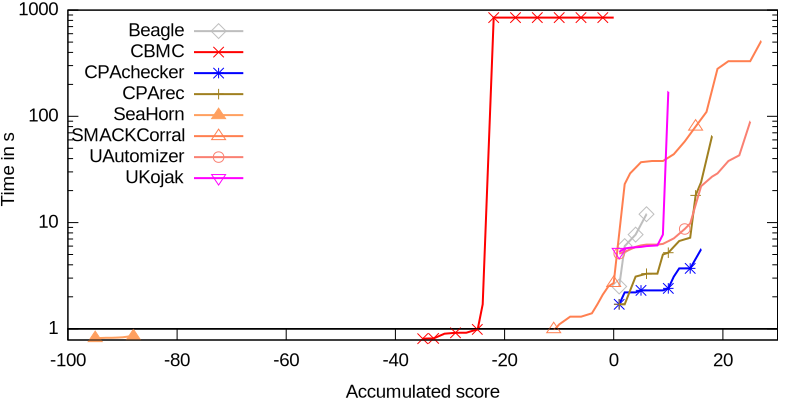
\includegraphics[width=\textwidth]{fig/competition-result}
  \caption{Accumulated Score over Time}
  \label{figure:accumulated-score}
\end{figure}


%%% Local Variables: 
%%% mode: latex
%%% TeX-master: "draft"
%%% LaTeX-command: "latex -shell-escape"
%%% End: 

\end{comment}
\chapter{Conclusion}\label{ch:conclusion}

In this work, we applied the \emph{probably-approximate-correct} (PAC) learning framework and its guarantee to the task of checking the validity of program assertions. More specifically, we propose the $\PAC$ guarantee, which is based on the guarantee provided by PAC learning. We proposed two approaches, the \emph{learning-based} and the \emph{sampling-based} approach, to handle the task. 

Both the learning-based and the sampling-based approaches utilize the $\PAC$ guarantee to provide correctness insurance of the program-under-test. The learning-based procedure makes use of a modified version of the automata learning framework mentioned in \cite{Angluin87}, which can handle the scenario when a target automaton contains an error, and replaces the checking of exact equivalence with sampling in order to provide programs with the $\PAC$ness guarantee. Moreover, the learning-based procedure incorporates several additional tests to enhance the performance. On the other hand, the sampling-based procedure directly takes the requirements $\PAC$ guarantee to calculate the number of samples necessary to provide programs with correctness insurance. It is also possible to execute the sampling-based procedure with several search strategies of the sampler.

We implemented a prototype named \PACMAN based on the two procedures. \PACMAN supports two modes, the \emph{synthesize-and-verify} mode and the \emph{direct} mode, implementing the learning-based and the sampling-based procedure respectively. We utilized several third-party components, such as software model checkers such as \textsc{CPAchecker} \cite{cpachecker} and CBMC \cite{cbmc}, the concolic tester \textsc{Crest} \cite{crest}, and the libraries CIL \cite{cil}, \textsc{libALF} \cite{libalf} and \textsc{libAMoRE++} \cite{libamore++}. In addition, we conducted experiments to determine the best learning algorithm and search strategy of the concolic tester with respect to performance. We submitted \PACMAN in \emph{direct} mode to participate in the recursive and array-reach subcategories of SV-COMP 2016 \cite{svcomp16}, and achieved promising results. Moreover, we submitted the learning-based procedeure to ICSE 2016 \cite{icse2016}, and was successfully accepted. 

Finally, it is possible to extend our approaches with different enhancement methods, such as applying heuristics, use sampling mechanisms with different distributions, etc. It is also viable to modify our learning-based approach so that it constructs automata approximating programs' function call graph instead of the control flow graph. With this work, we hope to find a balance between scalability and correctness guarantees by applying the PAC guarantee on the learning-based and sampling-based procedures, thus blurring the dichotomy between program testing and formal methods. 


\begin{comment}
% Extension: using program analyzer + bounded model checking

The number of iterations is perhaps the most important factor in our
recursion analysis technique (Table~\ref{table:experiments}) as it would
determine how many times of unwinding are applied.
We find that \textsc{CPAchecker} performs poorly when checking programs
that is unwound many times.
We however do not enable the more efficient block encoding in
\textsc{CPAchecker} for the ease of implementation.
One can improve the performance of our algorithm with the efficient but
complicated block encoding.
A bounded analyzer may also speed up the verification of bounded properties.

Our algorithm extracts function summaries from inductive invariants.
There are certainly many heuristics to optimize the computation of
function summaries.
For instance, some program analyzers return error traces when properties fail.
In particular, a valuation of formal parameters is obtained when
\textmd{CheckSummary} (Algorithm~\ref{algorithm:check-summary}) returns $\FF$.
If the valuation is not possible in the $\fun{main}$ function, one can use
its inductive invariant to refine function summaries.
We in fact exploit error traces computed by \textsc{CPAchecker} in the
implementation.

Another improvement on our algorithm is on selecting locations for extracting
inductive invariants.
In Algorithm~\ref{algorithm:mark-locations}, we select only outermost pairs of
locations for calls to the same function.
This is based on the observation that the unwound bodies of these function calls
contain more execution paths,
and hence their behaviors should be closer to the original function.
However, the extracted invariants in $s_i$ may be too precise to those certain
function calls and result in too coarse summary candidates constructed by
implication connective,
and consequently the candidates can not pass \textmd{CheckSummary} due to inner
function calls are not properly approximated.
Therefore, heuristics that select some locations of inner function calls may help
compute summary candidates with better quality.

Further enhancement and application of our work would be supporting recursive
data structures and verifying operations on the data structure.
Common recursive functions in real world C program mostly are simple operations
on recursive data structures, such as list, tree, graph, etc.,
but our prototype currently only verifies integer programs.
If our approach is adapted to handle data structures, a dedicated logic is
required for describing data structure as well as semantic for the operations,
and a \method{BasicAnalyzer} providing inductive invariants in such logic surely
is necessary.
Our primitive study reveals several difficulties on applying our approach with
separation logic~\cite{Reynolds02} and the \textsc{Thor}
analyzer~\cite{MagillTLT08}.

One major obstacle comes from \textmd{ComputeSummary} and \textmd{CheckSummary}.
In our method, implication connective and universal quantification are used to
derive summary.
These operators are intuitive in propositional and Presburger arithmetic logic.
By contrast, there is no such operator on separation logic.
Consequently, we tried to devise different methods for compute and check
summaries in order to avoid the usage of the operators.
A possible workaround for this problem is to use multiple formulae instead of
one single formula to represent one function summary.

Another problem arises from the expression allowed in $\mathtt{assume}$ and
$\mathtt{assert}$ command.
Our program model does not introduce a separated \emph{assertion language} for
specifying preconditions and postconditions,
and this is to comply with the assertions in C language.
The drawback of this choice is that the expressiveness and grammar of allowed
boolean expression in program is limited,
and hence not necessarily consistent with the logic in \method{BasicAnalyzer}.
To precisely describe a recursive data structure, we tried to introduce
annotations recognized by \method{BasicAnalyzer} into C programs.
In our study, we actually used the assertion language defined by \textsc{Thor}
to annotate C programs,
and much more efforts are needed to understand the underlying analyzer,
not to mention the transformation on the formulae.

Finally, reducing program features via program transformation techniques is the
core concept of our work.
We believe this idea can be applied to deal with other kinds of program
features, such as pointers, unbounded integral types, procedure calls through
dynamic look up, absent code due to external libraries, etc.
Program analysis tools can rely on one efficient and simple core
\method{BasicAnalyzer} and modular components doing transformation for different
program features.
The development tasks for the tools could be easily divided and dispatched,
and optimization for different components could be independent and loosely
coupled.
Overall, we believe the concept could speed up the process of research as well
as implementation on program analysis.

\end{comment}
\end{doublespace}

\backmatter
% Bibliography
\begin{doublespace}
\printbibliography
\end{doublespace}

\clearpage\end{CJK*}
\end{document}
